\documentclass [11pt]{report}
\usepackage [spanish] {babel}
\usepackage [T1]{fontenc}
\usepackage {ucs}
\usepackage [utf8]{inputenc}
\usepackage {anysize}
\usepackage {url}
\usepackage {graphicx}
\usepackage [colorlinks=true,linkcolor=black]{hyperref}
\usepackage {fancyvrb}
\usepackage {color}

\newcommand\PYZat{@}
\newcommand\PYZlb{[}
\newcommand\PYZrb{]}
\newcommand\PYbh[1]{\textcolor[rgb]{0.00,0.50,0.00}{\textbf{#1}}}
\newcommand\PYbg[1]{\textcolor[rgb]{0.73,0.40,0.53}{\textbf{#1}}}
\newcommand\PYbf[1]{\textcolor[rgb]{0.40,0.40,0.40}{#1}}
\newcommand\PYbe[1]{\textcolor[rgb]{0.73,0.13,0.13}{#1}}
\newcommand\PYbd[1]{\textcolor[rgb]{0.00,0.50,0.00}{\textbf{#1}}}
\newcommand\PYbc[1]{\textcolor[rgb]{0.40,0.40,0.40}{#1}}
\newcommand\PYbb[1]{\textcolor[rgb]{0.00,0.00,0.50}{\textbf{#1}}}
\newcommand\PYba[1]{\textcolor[rgb]{0.00,0.50,0.00}{\textbf{#1}}}
\newcommand\PYaJ[1]{\textcolor[rgb]{0.69,0.00,0.25}{#1}}
\newcommand\PYaK[1]{\textcolor[rgb]{0.73,0.13,0.13}{#1}}
\newcommand\PYaH[1]{\textcolor[rgb]{0.10,0.09,0.49}{#1}}
\newcommand\PYaI[1]{\fcolorbox[rgb]{1.00,0.00,0.00}{1,1,1}{#1}}
\newcommand\PYaN[1]{\textcolor[rgb]{0.74,0.48,0.00}{#1}}
\newcommand\PYaO[1]{\textcolor[rgb]{0.00,0.00,1.00}{\textbf{#1}}}
\newcommand\PYaL[1]{\textcolor[rgb]{0.00,0.00,1.00}{#1}}
\newcommand\PYaM[1]{\textcolor[rgb]{0.73,0.73,0.73}{#1}}
\newcommand\PYaB[1]{\textcolor[rgb]{0.00,0.50,0.00}{#1}}
\newcommand\PYaC[1]{\textcolor[rgb]{0.00,0.25,0.82}{#1}}
\newcommand\PYaA[1]{\textcolor[rgb]{0.00,0.63,0.00}{#1}}
\newcommand\PYaF[1]{\textcolor[rgb]{0.63,0.00,0.00}{#1}}
\newcommand\PYaG[1]{\textcolor[rgb]{1.00,0.00,0.00}{#1}}
\newcommand\PYaD[1]{\textcolor[rgb]{0.67,0.13,1.00}{#1}}
\newcommand\PYaE[1]{\textcolor[rgb]{0.25,0.50,0.50}{\textit{#1}}}
\newcommand\PYaZ[1]{\textcolor[rgb]{0.73,0.13,0.13}{#1}}
\newcommand\PYaX[1]{\textcolor[rgb]{0.73,0.13,0.13}{#1}}
\newcommand\PYaY[1]{\textcolor[rgb]{0.00,0.50,0.00}{#1}}
\newcommand\PYaR[1]{\textcolor[rgb]{0.40,0.40,0.40}{#1}}
\newcommand\PYaS[1]{\textcolor[rgb]{0.10,0.09,0.49}{#1}}
\newcommand\PYaP[1]{\textcolor[rgb]{0.00,0.00,0.50}{\textbf{#1}}}
\newcommand\PYaQ[1]{\textcolor[rgb]{0.49,0.56,0.16}{#1}}
\newcommand\PYaV[1]{\textcolor[rgb]{0.82,0.25,0.23}{\textbf{#1}}}
\newcommand\PYaW[1]{\textcolor[rgb]{0.00,0.00,1.00}{\textbf{#1}}}
\newcommand\PYaT[1]{\textcolor[rgb]{0.25,0.50,0.50}{\textit{#1}}}
\newcommand\PYaU[1]{\textcolor[rgb]{0.50,0.00,0.50}{\textbf{#1}}}
\newcommand\PYaj[1]{\textcolor[rgb]{0.10,0.09,0.49}{#1}}
\newcommand\PYak[1]{\textcolor[rgb]{0.25,0.50,0.50}{\textit{#1}}}
\newcommand\PYah[1]{\textcolor[rgb]{0.00,0.50,0.00}{#1}}
\newcommand\PYai[1]{\textcolor[rgb]{0.63,0.63,0.00}{#1}}
\newcommand\PYan[1]{\textbf{#1}}
\newcommand\PYao[1]{\textcolor[rgb]{0.67,0.13,1.00}{\textbf{#1}}}
\newcommand\PYal[1]{\textcolor[rgb]{0.73,0.40,0.53}{#1}}
\newcommand\PYam[1]{\textcolor[rgb]{0.00,0.50,0.00}{\textbf{#1}}}
\newcommand\PYab[1]{\textit{#1}}
\newcommand\PYac[1]{\textcolor[rgb]{0.73,0.13,0.13}{#1}}
\newcommand\PYaa[1]{\textcolor[rgb]{0.50,0.50,0.50}{#1}}
\newcommand\PYaf[1]{\textcolor[rgb]{0.25,0.50,0.50}{\textit{#1}}}
\newcommand\PYag[1]{\textcolor[rgb]{0.40,0.40,0.40}{#1}}
\newcommand\PYad[1]{\textcolor[rgb]{0.73,0.13,0.13}{#1}}
\newcommand\PYae[1]{\textcolor[rgb]{0.40,0.40,0.40}{#1}}
\newcommand\PYaz[1]{\textcolor[rgb]{0.00,0.50,0.00}{\textbf{#1}}}
\newcommand\PYax[1]{\textcolor[rgb]{0.40,0.40,0.40}{#1}}
\newcommand\PYay[1]{\textcolor[rgb]{0.60,0.60,0.60}{\textbf{#1}}}
\newcommand\PYar[1]{\textcolor[rgb]{0.53,0.00,0.00}{#1}}
\newcommand\PYas[1]{\textcolor[rgb]{0.10,0.09,0.49}{#1}}
\newcommand\PYap[1]{\textcolor[rgb]{0.73,0.40,0.13}{\textbf{#1}}}
\newcommand\PYaq[1]{\textcolor[rgb]{0.00,0.50,0.00}{#1}}
\newcommand\PYav[1]{\textcolor[rgb]{0.40,0.40,0.40}{#1}}
\newcommand\PYaw[1]{\textcolor[rgb]{0.00,0.50,0.00}{\textbf{#1}}}
\newcommand\PYat[1]{\textcolor[rgb]{0.73,0.13,0.13}{\textit{#1}}}
\newcommand\PYau[1]{\textcolor[rgb]{0.10,0.09,0.49}{#1}}


\begin{document}
\author{Albert Llop}
\title{\Huge{\textbf{Proyecto de Fin de Carrera} \\ Pizarra Web Compartida}}
\maketitle
\newpage
\tableofcontents

\chapter{Trabajo Previo}
%!TEX root = /Users/simo/Documents/PFC/memoria/memoria.tex
\section{Especificaci\'on} % (fold)
\label{sec:especificacion}

Este proyecto surge de la necesidad de realizar presentaciones a distancia, mayoritariamente por videoconferencia. Las videoconferencias están en el día a día de las empresas, y dichas presentaciones suelen ir acompañadas de diferentes documentos, ya sean PowerPoint o PDF's. El realizar estas presentaciones a distancia genera una serie de problemas:

\begin{itemize}
	\item Cada \emph{usuario} ve el documento individualmente, por lo cual no hay una sincronía entre lo que todos ven. Cada uno puede estar mirando una hoja distinta, o a un punto distinto.
	\item A diferencia de en una presentación real, el ponente carece de una pizarra o una superficie donde hacer explicaciones cuando las diapositivas no son suficiente.
\end{itemize}

Estas dos carencias básicas hacen que se pierda un gran porcentaje del tiempo de dichas conferencias en \underline{forzar} esa sincronía, con explicaciones constantes de en qué diapositiva se está, o a qué punto mirar, o en simular dicha pizarra, con explicaciones verbales en vez de gráficas.

Este proyecto por tanto intenta ser una solución para dichas empresas (o cualquier usuario), de forma que se pueda disponer de ambas funcionalidades de forma sencilla y accesible. Se pretende explorar el mundo del desarrollo de aplicaciones web interactivas, profundizando en la comprensión de las capacidades de las tecnologías actuales, disponibles al público en los navegadores típicos.

\subsection{Limitaciones}
Considerando que el mayor uso de este software va a ser por parte de empresas u otras organizaciones, más que particulares, hace que se tengan que considerar una serie de limitaciones. Éstas son las básicas:

\begin{itemize}
	\item Las empresas generalmente no permiten instalar nuevo software en sus ordenadores.
	\item Hay que tener en cuenta que muchas empresas tienen instalados firewalls muy restrictivos.
	\item Los documentos no tienen porqué ser vistos por todo el mundo, debe de haber algún tipo de seguridad que permita que solo la gente adecuada pueda estar en la presentación.
\end{itemize}


\subsection{Funcionalidades}
Una vez definida los objetivos básicos que queremos alcanzar, y las restricciones, se pueden empezar a formalizar las funcionalidades. La solución más simple que cumpla las limitaciones, y que permita alcanzar dichas funcionalidades básicas, es la realización de una \textbf{web} que permita cargar documentos y dibujar sobre ellos de forma compartida con otros usuarios. Cualquier persona puede disponer de un explorador web, y generalmente funcionará a través del firewall. El tercer requisito se puede cumplir fácilemte, pues la seguridad web es un campo suficientemente desarrolado para ello. A continuación se numeran más detalladamente las funcionalidades que esta web ha de tener, separados en funcionalidades del sistema y de la pizarra en si.

\subsubsection{Funcionalidades del Sistema}
De entre las múltiples posibilidades a la hora de plantear el funcionamiento de la web, se ha considerado interesante estructurar la web como una ``comunidad'' en que, simplificando al máximo, los usuarios se registran, pueden subir sus documentos, e invitan a otros usuarios a que se unan a sus presentaciones. Por lo tanto:

\begin{description}
	\item[Gestión de Usuario] Se tiene que poder registrar, hacer login y salir. Todas las opciones tienen que ser modificables por el usuario, por ejemplo, la contraseña.
	\item[Gestión de Grupos] (Opcional) Poder crear grupos, invitar a usuarios a dichos grupos.
	\item[Gestión de Pizarras] Cada usuario tiene que poder crear sus pizarras (el concepto de pizarra y sus funcionalidades se detallan en la sección siguiente), editarlas, y eliminarlas. Tiene que poder invitar a otros usuarios y/o grupos a partizipar en esa pizarra.
	\item[Participación en otras Pizarras] Cada usuario tiene que poder ver las pizarras a las que ha sido invitado, acceder y salir de ellas. (Opcional) Rechazar y solicitar invitaciones.
\end{description}

\subsubsection{Funcionalidades de la Pizarra}
Se considera una pizarra como un lugar donde poder escribir, dibujar, al cual se le ha cargado unas imágenes de fondo, que se podrían considerar las diapositivas de una presentación. Una persona que tenga que hacer dos presentaciones a partir de dos archivos distintos, tendrá que crear dos pizarras distintas, e invitar a la gente adecuada. Se puede invitar a gente distinta en cada pizarra que se haya creado. La figura \ref{fig:concept1} es una representación básica de cómo se vería una pizarra en funcionamiento. Arriba habrían las herramientas de dibujo, y a la derecha la lista de usuarios conectados. Las funcionalidades deseadas para las pizarras son las siguientes:

\begin{figure}[ht]
\centering
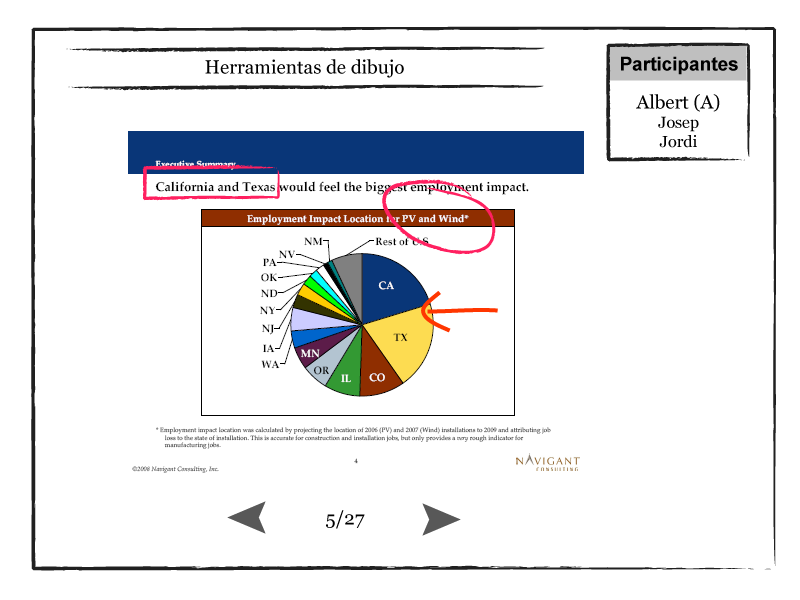
\includegraphics[width=16cm]{concepto.png}
\caption{Concepto básico de una pizarra}\label{fig:concept1}
\end{figure}

\begin{description}
	\item[Carga de documento] Cada pizarra tiene la posibilidad de añadir un documento que se cargará como imágenes de fondo. Dichas imágenes se pueden cargar de múltiples maneras.
	\begin{itemize}
		\item Una por una en formato de imagen JPG/PNG.
		\item Un zip/rar con el conjunto de imágenes.
		\item (Opcional) Mediante un PDF.
		\item (Opcional) Mediante una presentación PowerPoint directamente.
	\end{itemize}
	\item[Multipágina] Cada imagen tiene que ser una página diferente. Se tiene que poder avanzar y retroceder entre ellas.
	\item[Puntero] Se tiene que poder ver el puntero del ``administrador'', de forma que los usuarios pueden ver qué está señalando en ese momento, en vez de esperar a que dibuje un círculo, por ejemplo.
	\item[Herramientas de dibujo] Existen múltiples posibilidades para esto, y se intentarán implementar el máximo número posible, pero se establecen unos mínimos:
	\begin{description}
		\item[Lápiz] Con selección de color y grosor.
		\item[Lineas rectas] Con selección de color y grosor.
		\item[Texto] Con selección de color, fuente y tamaño. (Estos dos últimos opcionales)
		\item[Goma de borrar] Para poder eliminar objetos con la mayor sencillez posible.
		\item[Subrallador] (Opcional) Para todas las herramientas, poder seleccionar modo de subrallado, en que se harán los dibujos semitransparentes a modo de subrallador, en vez de sólidos.
		\item[Cajas y elipses] (Opcional)
		\item[Imágenes] (Opcional) Se desea la posibilidad de añadir imágenes extra, a parte de la del documento de fondo.
	\end{description}
	\item[Guardar] Se tiene que poder guardar la situación actual de la pizarra para cargarla posteriormente.
	\item[Formato en capas] (Opcional) Ya se entiende que cada pizarra tendrá dos capas, la de la imagen de fondo, y en la que se hagan todos los dibujos. Sería interesante hacer que se pueda dibujar por capas, crearlas, eliminarlas, moverlas arriba/abajo.
	\item[Exportar] Se tiene que poder exportar la situación de la pizarra en algun formato (pdf, imagen) y/o poder imprimirse.
	\item[Lista de usuarios] Listar los usuarios que están en ese momento conectados en la pizarra.
	\item[Chat] (Opcional) Posibilidad de establecer un chat entre los usuarios conectados. (Opcional) Poder guardar dicho chat junto con el estado de la pizarra.
\end{description}

\begin{figure}[h]
\centering
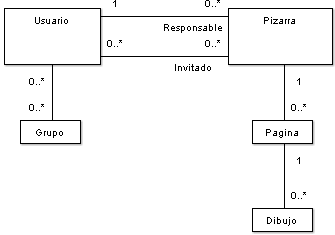
\includegraphics{Diagramadeclase1.png}
\caption{Diagrama de clases básico}\label{fig:diagramaclases}
\end{figure}

Para ayudar a entender el concepto de lo que será el sistema, la figura \ref{fig:diagramaclases} representa un diagrama de clases extremadamente simplificado.


\subsection{Tecnología}
Una explicación más detallada de la tecnología que se va a utilizar se podrá encontrar en las próximas secciones, pero hay una serie de requisitos que se afectan a la tecnología que se use, que deben ser considerados.

\begin{description}
	\item[Servidor] El servidor no tiene que requerir más de lo que sería un servidor web típico. Apache/MySQL sobre linux. Otros requisitos se admiten, pero tienen que estar accesibles de forma sencilla (binarios en forma de paquete, por ejemplo) para las distribuciones típicas de Linux. Nada de compilar fuentes, por ejemplo.
	\item[Cliente] Los navegadores más importantes tienen que estar soportados, Internet Explorer, Firefox y Safari como mínimo. Se intentará alcanzar el mayor grado de compatibilidad con Explorer 6, y en el peor caso, que cumpla las funcionalidades básicas.
	\item[Software] Puesto que los usuarios no tienen que tener que instalar ningún software nuevo, es altamente deseable que la web sea lo más sencilla posible. Se hará todo lo posible por evitar utilizar tecnologías que el usuario no tiene porqué tener instalados en su ordenador. Se va a intentar cumplir el requisito de que el usuario solo tiene que tener funcionando un navegador web moderno. En cuanto a la programación del esqueleto de la web, se considera interesante utilizar un lenguaje dinámico más moderno para agilizar el proceso, en vez del clásico PHP o ASP. También, el interés propio de explorar nuevas áreas, puesto que ya se tiene amplia experiencia con PHP, Ruby es un lenguaje muy interesante, y será considerado en la etapa de diseño.
\end{description}

\newpage
%!TEX root = /Users/simo/Documents/PFC/Chapter1/chapter1.tex
\section{Tecnolog\'ia} % (fold)
\label{sec:tecnologia}

Se ha decidido realizar una web con una serie de funcionalidades, pero incluso en ese entorno existen múltiples lenguajes y plataformas para todo tipo de desarrollos. Este documento pretende considerar las posibilidades existentes, y escoger la más adecuada para este proyecto a partir de una serie de criterios.

En un primer acercamiento se pueden diferenciar dos partes claras que forman este proyecto. Primero, el desarrollo de la pizarra, implementando el máximo de funcion:alidades establecidas en la especificación, y segundo, el desarrollo del sistema, con su gestión de usuarios, grupos y pizarras.

\subsection{Pizarra}
A la hora de considerar las posibles tecnologías que permitan implementar una pizarra de este tipo, aparecen múltiples opciones que, en mayor o menor medida, podrían funcionar. Sin embargo, en la especificación se ha definido que la solución debe ser accesible desde una página web, a través de firewalls rigurosos, y con el mínimo de \emph{software extra} posible. Ésto nos deja básicamente con tres posibles opciones, descartando muchos de los lenguajes más clásicos de programación, como podría ser C++.

Dichas opciones son \texttt{JavaScript}, \texttt{Flash/Shockwave} o \texttt{Java}. Otro tipo de aplicaciones como podría ser un \texttt{Control ActiveX} queda descartado desde el principio por su dificultad de ejecutar en exploradores que no sean Internet Explorer, y por estar aún más limitados que entornos restrictivos como son los ordenadores de las empresas. Los tres considerados son suficientemente conocidos, y están soportados por la gran mayoría de los ordenadores de hoy día.

Para poder hacer una comparativa objetiva entre ellos, los criterios a seguir serán los siguientes:

\begin{description}
	\item[Facilidad de implementación] Una tecnología que permita desarrollar de forma más rápida también permite desarrollar más y con menos errores.
	\item[Calidad del resultado] Es muy posible que con alguna tecnología el resultado que se llegue a obtener sea de mejor calidad por múltiples razones.
	\item[¿Accesible por todo el mundo?] ¿Es posible que algún usuario tenga alguna limitación que no le permita usar el programa debido al uso de esta tecnología?
	\item[Otras motivaciones] Se considerará también muy importante características como el ser una tecnología novedosa, algo con el que el autor aún no haya trabajado, tendencias de mercado, etc.
	\item[Viabilidad] Pueden haber razones por las cuales una tecnología es simplemente inviable, ya sean monetarias, de complejidad, adquisición de licencias, etc.
\end{description}


\subsubsection{Flash}
Adobe Flash (anteriormente Macromedia Flash) era originariamente un entorno enfocado al desarrollo de animaciones vectoriales, pero su gran popularidad ha hecho que se haya ido expandiendo hasta convertirse en una plataforma multimedia mucho más interactiva, gracias a \texttt{ActionScript}, el lenguaje mediante el cual se puede programar todo tipo de aplicaciones en flash.

\begin{description}
	\item[Facilidad de implementación] Es muy posible que de las tres tecnologías esta fuera la que permita una implementación más sencilla de la pizarra en si, pues Flash proporciona todas las herramientas necesarias para tratar los dibujos que se necesitan hacer. Un magnífico ejemplo de pizarra interactiva puede encontrarse en \url{www.imaginationcubed.com}. En cuanto a las funcionalidades de pizarra compartida, Flash ofrece \emph{Flash Media Server}\footnote{Adobe, Flash Media Server Products - \url{http://www.adobe.com/products/flashmediaserver/}}, que soluciona todas las necesidades de aplicaciones en tiempo real y compartición de objetos.
	\item[Calidad del resultado] Los resultados que se pueden obtener con flash en una aplicación interactiva de este tipo pueden ser más que satisfactorios. La calidad gráfica, así como la interactividad serán tan buenas como el programador/diseñador sea capaz.
	\item[¿Accesible por todo el mundo?] Flash es una tecnología muy extendida por todo el mundo, pero por desgracia suele utilizarse para aplicaciones que muchas empresas podrían considerar como inadecuadas en un espacio de trabajo (juegos en flash o youtube, por ejemplo). Si bien es cierto que la posibilidad de que un ordenador moderno no disponga de flash es muy reducida, no es algo imposible, y mucho menos en el contexto de las empresas.
	\item[Otras motivaciones] Flash es una tecnología que lleva muchos años en el mercado y que ha madurado considerablemente. Sin embargo suele requerir de capacidades de diseñador/animador más que de programador, por tanto no se considera muy adecuada para el perfil del autor.
	\item[Viabilidad] El mayor problema de Adobe Flash es el hecho de que es una tecnología cerrada. La licencia de Flash CS3 Profesional, necesario para desarrollar el programa, cuesta \$699\footnote{Adobe, Flash CS3 Professional - \url{http://www.adobe.com/products/flash/?ogn=EN_US-gntray_prod_flash_home}}, y la licencia para el servidor Flash Media Server asciende a \$4500\footnote{Adobe, Flash Media Interactive Server 3 - \url{http://www.adobe.com/products/flashmediainteractive/}}. Ambos productos están fuera del alcance en cualquier implementación realista. Si bien es cierto que el servidor de desarrollo es gratis, se considera importante que sea posible utilizar el software una vez acabado, si no por cualquier empresa, al menos por la mayoría.
\end{description}

\subsubsection{Java}
Java es un lenguaje de programación en toda regla, que ofrece la posibilidad de generar los llamados applets, enfocados al entorno web, con todas las ventajas (e inconvenientes) de un lenguaje de programación normal y corriente. Dichos applets son integrables en las webs sin problema, siempre y cuando el usuario tenga instalado la JVM (\emph{Java Virtual Machine}).

\begin{description}
	\item[Facilidad de implementación] Java permite hacer prácticamente cualquier cosa, el único problema es que no es un lenguaje pensado especialmente para aplicaciones interactivas como en este caso. Además, para que dichos applets interactúen con el sistema, y por ejemplo, se puedan guardar pizarras, sería conveniente que se funcionase con Servlets y JSP's, lo cual no lo hace más difícil, pero si más restrictivo.
	\item[Calidad del resultado] Al no ser un lenguaje pensado para este tipo de aplicaciones, es posible que el resultado no sea de la calidad que se espera, muy pesado y engorroso para el usuario por tener que cargar el applet. Java suele utilizarse para programas más grandes, o que necesitan de mayor procesado que lo necesario por una pizarra interactiva.
	\item[¿Accesible por todo el mundo?] De forma similar al flash, java está instalado en la mayoría de ordenadores personales, aunque es posible que en menor medida.
	\item[Otras motivaciones] El autor ya ha realizado numerosas aplicaciones en java, incluyendo applets, así como servlets y JSP's, con lo cual se considera poco interesante repetir la experiencia.
	\item[Viabilidad] A pesar de lo que parecen ser numerosos problemas, Java sería una opcion perfectamente factible, dentro de las capacidades del autor, y que resultaría en un programa quizá no tan agradable visualmente como si funcional. Se puede desarrollar en java de forma libre, no habría ningún gasto extra, ni problema de licencias.
\end{description}

\subsubsection{JavaScript}
JavaScript, a diferencia de las otras opciones, es un lenguaje interpretado por los navegadores que permite la ejecución de, en principio, pequeñas acciones dentro de la página web. Dichas acciones pueden ser desde hacer pequeñas operaciones con datos introducidos en un campo de texto, habilitar o desabilitar elementos web, hasta otras cosas mucho más complejas. Javascript es en realidad un lenguaje muy completo que permite hacer una gran variedad de cosas, y esto se ha ido demostrando conforme han ido pasando los años. Ejemplos de webs con un gran uso de javascript podrían ser, por ejemplo, google docs\footnote{Google Docs - \url{http://docs.google.com}} o google mail\footnote{Google Mail - \url{http://mail.google.com}}.

\begin{description}
	\item[Facilidad de implementación] Por desgracia, Javascript se ha utilizado mayoritariamente para pequeñas operaciones como las descritas anteriormente, lo cual ha hecho que haya, en general, poca experiencia a la hora de desarrollar aplicaciones más complejas con él, y lo que ello conlleva (falta de documentación, ejemplos, librerías, etc). Otro problema bastante grande, es el hecho de que sea un lenguaje interpretado por el explorador, y que no todos los exploradores tengan una implementación similar de Javascript. A pesar de los esfuerzos del W3C\footnote{World Wide Web Consortium - \url{http://www.w3c.org}} aún hay diferencias entre implementaciones. Ésto hace que se tengan que tener en cuenta más factores a la hora de programar, haciendo el proceso más complicado.	
	\item[Calidad del resultado] Javascript permite crear aplicaciones muy ágiles para el usuario, utilizando técnicas ya extendidas como Ajax (Asynchronous JavaScript And XML), creando una experiencia de usuario muy positiva. Si bien no está pensado para realizar aplicaciones gráficas, existen ejemplos funcionales de una pizarra similar a la que se quiere implementar, usando Javascript. Existen librerías que permiten trabajar con formas sencillas, como podría ser jsgraphics\footnote{High Performance JavaScript Vector Graphics Library - \url{http://www.walterzorn.com/jsgraphics/jsgraphics_e.htm}}, aunque se intentará encontrar alguna solución mejor.
	\item[¿Accesible por todo el mundo?] Ésta es la tecnología que más personas podrán disfrutar. Solamente hace falta tener un navegador relativamente moderno (Internet Explorer 6+, Mozilla Firefox, Safari, y muchos otros), sin ningún tipo de añadido. El problema reside en el programador, por crear código que sea entendible por todos, no en el usuario.
	\item[Otras motivaciones] Javascript está en auge en estos momentos, se está por fin dando un uso completo a todo su potencial por numerosas compañías, y los resultados son más que sorprendentes. La agilidad de las aplicaciones hace que se empiece a utilizar la web para múltiples tareas que antes estaban relegadas solamente a programas individuales. Existen implementaciones de todo tipo de aplicaciones con javascript, desde clientes de mensajería instantánea, a videojuegos, pasando por clientes de correo, procesadores de texto u hojas de cálculo. El autor aún no ha trabajado con este lenguaje más que en contadas ocasiones y de forma mínima, haciéndolo muy atractivo a la hora de desarrollar un proyecto como este.
	\item[Viabilidad] No hay ninguna razón que haga el uso de javascript inviable, existen pizarras compartidas online ya implementadas con gran éxito, pero no cumplen los requisitos que este proyecto se ha planteado, o son cerradas/de pago.
\end{description}

\subsubsection{Conclusión}
Después de considerar los criterios que se han establecido, se ha decidido utilizar \texttt{Javascript} como técnica para implementar la Pizarra. Flash hace bastante inviable su desarrollo por el alto costo de sus licencias, y aunque se puedan usar licencias de prueba, el producto final sería inviable de utilizar por cualquier empresa que no disponga ya de las licencias de Flash Media Server, y por supuesto totalmente imposible en caso de querer ponerla en funcionamiento por parte del autor. En cuanto a Java, es una solución interesante, y que funcionaría sin demasiados problemas, pero se pretende que sea algo ágil, que cualquiera pueda utilizarlo, y Java suele tener problemas con ello. Javascript es interesante en todos los aspectos, y se considera que permitirá realizar una implementación excelente, además de servir para profundizar más los conocimientos del autor en la materia web actual.

\subsection{Sistema}
Hasta ahora se ha considerado solamente cómo implementar las Pizarra, que si bien es el elemento más importante del proyecto, no es el único. Las funcionalidades que se han definido requieren de otro tipo de lenguajes, de los cuales hay una gran variedad, y se considerarán a continuación bajo los siguientes criterios, similares al apartado anterior.

\begin{description}
	\item[Facilidad de implementación]
	\item[Calidad del resultado]
	\item[Disponibilidad en servidores comunes] 
	\item[Otras motivaciones]
	\item[Viabilidad]
\end{description}

Las opciones a considerar serán \texttt{PHP}, \texttt{JSP/Servlets Java} y \texttt{Ruby}. Existen múltiples lenguajes que permiten programar webs dinámicas, como podrían ser python, perl, o incluso C. Sin embargo no son tan populares en cuanto a desarrollo web se refiere, por lo tanto solamente se considerarán las que son mayoritarias actualmente.

\subsubsection{PHP}
PHP se describe a si mismo como\footnote{\url{http://www.php.net}}:
\begin{quote}
\emph{PHP  is a widely-used general-purpose scripting language that is especially suited for Web development and can be embedded into HTML.}
\end{quote}

PHP se ha convertido en el lenguaje de scripting más popular en la actualidad, utilizado en más de 20 millones de sitios web\footnote{PHP Usage Stats - \url{http://www.php.net/usage.php}}. Ésto, añadido a su licencia libre, hace que exista una comunidad enorme, con todos los beneficios que ello conlleva.

PHP permite generar contenido dinámicamente en el servidor, dependiendo de las numerosas variables existentes. Se pueden ``incrustar'' trozos de código PHP en el html de forma que PHP genere ese contenido haciendo las operaciones necesarias, como por ejemplo, consultando una base de datos.

\begin{description}
	\item[Facilidad de implementación] PHP se considera un lenguaje simple que permite desarrollar sitios de tamaño pequeño o medio con relativa simplicidad. Existen múltiples scripts ya programados que incluso podrían llegar a ayudar en el proceso de implementación del sistema.
	\item[Calidad del resultado] El amplio uso de PHP en sitios web hace que sea un sistema completamente depurado con mínimos agujeros de seguridad, lo cual ayudado por la gran cantidad de documentación de que se dispone, hace que las webs resultantes no tengan nada que envidiar a las producidas por otros lenguajes. Realmente el límite está en manos del programador, no del lenguaje.
	\item[Disponibilidad en servidores comunes] PHP viene con cualquier distribución de linux hoy día, y se puede instalar en prácticamente cualquier sistema operativo.
	\item[Otras motivaciones] El autor de este proyecto ya tiene amplia experiencia en la programación de webs con PHP. No aportaría ningún conocimiento nuevo, más que incrementar la experiencia ya existente.
	\item[Viabilidad] Este proyecto en PHP sería totalmente viable.
\end{description}

\subsubsection{JSP/Servlets Java}
JSP (JavaServer Pages) se puede considerar como una abstración de los Servlets, en un lenguaje más alto. Un JSP se compila generando un servlet, que es código Java, el cual se vuelve a compilar con un compilador Java tradicional.

Simplificando, JSP funciona de forma muy similar a PHP, pero con todo el soporte de Java, y lo que ello conlleva. Hace que sea posible utilizar cualquier clase Java para generar contenidos dinámicos, de la misma forma que PHP usa sus librerías.

\begin{description}
	\item[Facilidad de implementación] JSP es tan simple como Java, y tiene todas las características necesarias para hacer cualquier sitio web. Sin embargo, Java no está tan enfocado a páginas webs como podría ser PHP. Se tiene una gran ventaja en el hecho de que se puede usar cualquier código Java, por tanto, cualquier librería ya hecha, pero también es cierto que al no ser enfocado principalmente a páginas web, pueda hacer tareas comunes (contactar con la base de datos), mucho más engorrosas.
	\item[Calidad del resultado] JSP tiene todo lo necesario para realizar una web de calidad.
	\item[Disponibilidad en servidores comunes] La instalación y configuración de un servidor típico apache para funcionar con JSP's suele requerir más trabajo que con PHP, pues no suele instalarse de forma automática, y requiere de trabajo extra por parte del administrador. Apache Tomcat\footnote{Apache Tomcat - \url{http://tomcat.apache.org}} es implementación oficial de JSP y Java Servlets, y suele ser bastante fácil de encontrar para las respectivas distribuciones. 
	\item[Otras motivaciones] El autor ya ha realizado un proyecto utiliazndo JSP y Java Servlet, si bien no en profundidad, ya conoce las características principales. Sería interesante (o casi imprescindible) si se hubiera decidido usar un Applet Java para el desarrollo de la Pizarra.
	\item[Viabilidad] Este proyecto sería totalmente viable utilizando JSP y Servlets Java, incluso si se utiliza Javascript o Flash para la implementación de las Pizarras.
\end{description}

\subsubsection{Ruby}
Ruby es un lenguaje que está en auje desde hace relatiamente poco, por numerosas razones. La más importante de ellas sea probablemente la plataforma Rails\footnote{Ruby on Rails - \url{http://www.rubyonrails.org/}} (de ahí el conocido Ruby on Rails), que simplifica el proceso de generación de código de forma drástica. Existen numerosos ejemplos en forma de screencasts demostrando la implementación de aplicaciones simples en tiempos menores a 15 minutos\footnote{Screencasts of Ruby on Rails, Creating a weblog in 15 minutes - \url{http://www.rubyonrails.org/screencasts}}.

\begin{description}
	\item[Facilidad de implementación] Ésta es la característica estrella de Ruby on Rails. Simplifica todas las tareas repetitivas a la hora de desarrollar aplicaciones web con un fondo de base de datos, es decir, la mayoría. Lo único que puede dificultar la implementación es la falta de experiencia del autor con esta plataforma.
	\item[Calidad del resultado] El resultado tendrá la misma calidad que el realizado por cualquier otro lenguaje de scripting. Hay argumentos que defienden la mayor calidad de las webs realizadas en ruby por su grandísima simplicidad, lo cual ayuda a una futura expansión mucho más sencilla.
	\item[Disponibilidad en servidores comunes] Ruby se encuentra cada vez más fácilmente en las distribuciones típicas de linux. La forma de configurar un servidor Apache para soportar Ruby es similar a la de cualquier otro lenguaje de scripts, como podría ser Perl. Hace falta tener los paquetes necesarios en el servidor (ruby y rails) y a partir de ahí hay varias formas de hacer que Apache pueda soportar proyectos en rails. Una de las soluciones, por ejemplo, necesita que tenga los módulos rewrite y fcgi activados. Otra solución es más sencilla, pero requiere compilar el módulo.
	\item[Otras motivaciones] Hoy por hoy existe una gran expectación en cuanto a Ruby on Rails. Cada vez más webs se desarrollan con esta tecnología, y eso se demuestra en que cada vez más se pueden encontrar empresas de hosting con soporte para Rails. No hay ninguna razón objetiva para apoyar todas estas consideraciones, es posible que Rails no deje de ser una plataforma minoritaria, pero a día de hoy, tiene un crecimiento muy marcado que lo convierte en una plataforma muy atractiva a la hora de profundizar los conocimientos del autor en temas de desarrollo web.
	\item[Viabilidad] No hay ninguna razón para que este proyecto no sea viable bajo Ruby.
\end{description}

\subsubsection{Conclusión}
En este apartado las tres opciones que se han considerado son prácticamente igual de competentes. Si bien Ruby tiene más posibilidades de conseguir un desarrollo más rápido y de mayor calidad, es también el que necesitará más tiempo de aprendizaje. Debido a que las tres opciones son prácticamente equivalentes en cuanto a viabilidad se refiere, Ruby será en lenguaje escogido para este proyecto, como principal razón el interés del autor en estudiar áreas nuevas del desarrollo web.

\subsection{Entendiendo las Tecnologías}
El desarrollo de una página web no se puede tomar como el desarrollo de una aplicación cualquiera. Para este proyecto se han diferenciado dos partes que deberán seguir un desarrollo independiente antes de juntarse. El desarrollo de la pizarra si puede plantearse de forma similar a una aplicación, siempre teniendo en cuenta las grandes limitaciones que javascript impone. Es por eso que se considera importante entender lo máximo posible el lenguaje antes de empezarse a plantear como será el proceso de diseño, y posterior implementación.

No hay que olvidar tampoco, que gracias a que Ruby, o más concretamente Rails, ofrece una gran cantidad de opciones para automatizar tareas comunes en el desarrollo web, incluyendo pequeños trozos de javascript, también se intentará entender cual es el funcionamiento de Ruby, qué oportunidades ofrece Rails, y cómo puede ayudar en el desarrollo de la Pizarra.

En cuanto al desarrollo del sistema de la web, se seguirán los procesos típicos para ello, en este caso enfocado a Ruby on Rails, y las facilidades que nos aporta. Ruby on Rails, al fin y al cabo, considera que revoluciona la forma en que se desarrollan webs hoy día \footnote{Quotes about Ruby on Rails - \url{http://www.rubyonrails.org/quotes}}, por tanto conviene ver de qué tipo de revolución se está hablando.

\subsubsection{Javascript}
Las características básicas se han descrito anteriormente, pero es necesario entender más profundamente como funciona, y cual es el proceso típico de desarrollo de un javascript, para poder planear el desarrollo de la Pizarra. Se quiere evitar empezar a escribir código ciegamente sin tener un entendimiento previo de qué se está manejando.

\textbf{Orientado a Objetos}
El primer detalle importante sobre Javascript, es que es orientado a objetos. Cada elemento de una página se considera un objeto, y siempre existe una manera de acceder a él. Por ejemplo, si se tuviera una imagen definida así:
\begin{verbatim}
<img src="foo.jpg0" name="imagen1">
\end{verbatim}

Se podría acceder a su atributo \texttt{src} mediante:

\begin{verbatim}
document.images['imagen1'].src
\end{verbatim}

Es decir, existe el objeto \texttt{document}, que simboliza toda la página web, mediante el cual se accede al atributo \texttt{images}, que engloba todas las imágenes, el cual es un vector, y es posible acceder al que tiene de nombre ``imagen1'', y de ahí se accede al atributo \texttt{src}.

Mozilla Developer Center contiene un artículo\footnote{Introduction to Object-Oriented JavaScript - \url{http://developer.mozilla.org/en/docs/Introduction_to_Object-Oriented_JavaScript}} donde se explican todas las características de orientación a objetos en javascript, y como implementarlas con un ejemplo muy claro. Tiene una forma un tanto peculiar de crear y heredar elementos, pero es posible trabajar sin problemas, teniendo en cuenta que javascript no soporta herencias múltiples.

\textbf{Librería gráfica}
Es importante recordar que Javascript es un lenguaje de scripting sin ningún tipo de soporte para gráficos incorporado. Entendiéndolo de una forma lo más abstracta posible, lo que permite es tomar la página web como un documento de texto con formato (generalmente) XML, y realizar acciones sobre este texto (modificándolo por ejemplo), apoyándose en otras funciones del explorador. Dichas funciones podrían ser, consultar lo que el usuario ha introducido en formularios, acceder a variables del explorador (para saber la IP del usuario o el navegador que usa, por ejemplo), o lanzar pequeños avisos en forma de ventana de aviso. La mencionada anteriormebte técnica Ajax permite acciones un poco más elaboradas, como por ejemplo,consultar otras páginas (que contiene una lista los usuarios de una base de datos), y actuar acordemente (mostrando esa lista de usuarios en la página actual, sin haber tenido que recargar la página entera).

Así pues, si se quiere tratar con gráficos, hay que buscar una solución en la que Javascript pueda realizarlos modificando texto. La librería que se ha encontrado, jsgraphics\footnote{High Performance JavaScript Vector Graphics Library - \url{http://www.walterzorn.com/jsgraphics/jsgraphics_e.htm}}, soluciona esto generando múltiples elementos div de 1 pixel de tamaño. No son imágenes, pero visualmente lo parecen.

En busca de otras opciones para realizar esta función, se ha decidido investigar implementaciones actuales de aplicaciones web que realicen dibujos semejantes a los que se quieren lograr en este proyecto. Existen diversas implementaciones usando la librería mencionada anteriormente, pero gracias a skrbl\footnote{skrbl: easy to share online whiteboard\url{http://www.skrbl.com/}}, se ha descubierto otra opción muy interesante.

Los elementos que se quieren dibujar para este proyecto son perfectamente implementables por lo que se conoce como gráficos vectoriales. Círculos, líneas, cuadrados, texto, todo esto se puede hacer de forma sencilla con cualquier programa que permita editar este tipo de gráficos. Existe un formato abierto llamado SVG\footnote{Scalable Vector Graphics - \url{http://www.w3.org/Graphics/SVG/}}, cuyo formato no es binario como suelen ser los propietarios, sino especificado en XML. Gracias a esto, es posible crear y modificar gráficos vectoriales mediante Javascript. Un ejemplo de archivo SVG podría ser el de la figura \ref{fig:svg_example} (ejemplo extraido de Wikipedia)

\begin{figure}[ht]
\centering

\includegraphics{svg_example.png}
\begin{verbatim}
<?xml version="1.0"?>
<!DOCTYPE svg PUBLIC "-//W3C//DTD SVG 1.1//EN"
                     "http://www.w3.org/Graphics/SVG/1.1/DTD/svg11.dtd">
<svg xmlns="http://www.w3.org/2000/svg" version="1.1" width="467" height="462">
 
  <!-- This is for the red square -->
  <rect x="80" y="60" width="250" height="250" rx="20" fill="red"
         stroke="black" stroke-width="2px" />
  <!-- This is for the blue square -->
  <rect x="140" y="120" width="250" height="250" rx="40" fill="blue"
        fill-opacity="0.7" stroke="black" stroke-width="2px" />
</svg>
\end{verbatim}
\caption{Ejemplo simple de archivo svg}\label{fig:svg_example}
\end{figure}

Por desgracia, realizando pruebas sobre cómo se incluyen gráficos SVG en páginas web, se observa que dichos gráficos no funcionan en ninguna versión de Internet Explorer (Firefox y Safari funcionan sin problemas). Se descubre que es necesario un plugin para poder visualizar dichos archivos en este navegador, pero sin embargo se puede utilizar skrbl sin ningún problema. Se acaba descubriendo otro formato llamado VML\footnote{Vector Markup Language - \url{http://www.w3.org/TR/1998/NOTE-VML-19980513}}. El siguiente párrafo introductorio de la entrada sobre VML en la Wikipedia\footnote{Vector Markup Language, Wikipedia - \url{http://en.wikipedia.org/wiki/Vector_Markup_Language}} explica perfectamente porqué no funcionan los SVG en Internet Explorer:

\begin{quote}
	\textbf{Vector Markup Language (VML)} is an XML language used to produce vector graphics. VML was submitted as a proposed standard to the W3C in 1998 by Microsoft, Macromedia, and others, but was rejected as a web standard because Adobe, Sun, and others submitted a competing proposal known as PGML. The two standards were joined to create SVG.

Even though rejected as a standard by the W3C, and largely ignored by developers, Microsoft still implemented VML into Internet Explorer 5.0 and higher and in Microsoft Office 2000 and higher.
\end{quote}

A pesar de no ser la solución ideal, todos los Internet Explorer con versión 5.5 o superior implementan este lenguaje, con un formato similar al SVG. Es posible, por tanto, tratar con gráficos vectoriales en los navegadores mayoritarios (los que interesa en este proyecto), gracias a estos dos formatos. 

\textbf{Canvas}
Estas dos no son las únicas formas de tratar con gráficos vectoriales en páginas web. En la nueva especificación HTML (versión 5\footnote{W3C, HTML5 - \url{http://www.w3.org/html/wg/html5/}}, actualmente aún en formato borrador aún), se especifica un nuevo elemento, denominado \texttt{<canvas>}, y cuyo objetivo es la representación gráficos vectoriales directamente en la web. Es independiente de VML o SVG, y ya está implementado en los navegadores mayoritarios, excepto Internet Explorer. Existe, sin embargo, una librería en javascript\footnote{Explorer Canvas - \url{http://excanvas.sourceforge.net/}}, que automáticamente transforma cualquier elemento \texttt{<canvas>} en su equivalente en VML, por lo cual se puede considerar que es soportado en todos los exploradores mayoritarios actuales.

El funcionamiento de canvas es completamente distinto al de SVG y VML. Se basa en considerar que hay un puntero que puede ir haciendo diversos tipos de trazos. Se puede mover a cualquier punto dentro de un área definida, y moverse hacia otro haciendo el dibujo. Existen funciones para hacer todo tipo de ``trazos'', permitiendo dibujar líneas, círculos, y todo lo necesario.

Este tipo de planteamiento, sin embargo, no es adecuado para el tipo de aplicación que se pretende desarrollar. En el caso de la pizarra, existirán diferentes elementos que se irán añadiendo, quitando y modificando. El formato SVG o VML es ideal, puesto que está formado por dichos elementos, y para por ejemplo, crear un círculo, simplemente se añade una nueva etiqueta correspondiente a un círculo. En el caso de Canvas, sin embargo, habría que redibujar todo desde el principio, incluyendo el trazo final de un círculo. Básicamente, cada vez que se modifique algo en canvas, hay que redibujar todo de nuevo.

Por lo tanto, canvas es ideal para realiar dibujos estáticos, pero poco adecuado para realizar aplicaciones interactivas como será ésta.

\subsubsection{Ruby}
Ruby es un lenguaje inspirado en Perl, Smalltalk, Eiffel, Ada y Lisp, creado por Yukihiro ``matz'' Matsumoto\footnote{Acerca de Ruby - \url{http://www.ruby-lang.org/es/about/}}. Ruby en si es solo el lenguaje, y existen diferentes implementaciones. De ellas, la oficial está implementada en \texttt{C} y es interpretado en una sola pasada\footnote{Ruby, Wikipedia - \url{http://es.wikipedia.org/wiki/Ruby}}. Típicamente se puede ejecutar un archivo ruby desde la línea de comandos, con una linea parecida a la siguiente:

\begin{verbatim}
$ ruby archivo.rb
\end{verbatim}

\textbf{Desarrollando la web, Ruby on Rails}
Rails\footnote{Ruby on Rails - \url{http://www.rubyonrails.org/}} es una plataforma de desarrollo web basada en Ruby, que ayuda a desarrollar aplicaciones web, y que sigue el paradigma Modelo Vista Controlador. Dicho patrón es muy semejante al conocido patrón en 3 capas, separando la capa que trata con los datos, la que realiza operaciones, y la del interfaz. Rails es capaz de hacer la representación del modelo (dominio) por nosotros, simplemente observando la base de datos actual, genera los controladores para manejar los elementos (crear, borrar, modificar, listar, etc) y las vistas correspondientes a cada una de dichas operaciones. A partir de ahí, el programador solo debe modificar a su gusto lo que rails ha generado.

Este proceso de desarrollo hace que sea relativamente sencillo de adaptar al proceso típico de desarrollo de una pieza de software tradicional. Es posible empezar por especificar las clases del dominio, traducirlo a una base de datos, y dejar que Rails cree toda la estructura. A partir de ahí se puede empezar a implementar código obviando partes laboriosas como son las de tratar con la base de datos. Ahora se dispone de unas clases en Ruby, para cada clase del dominio, con una serie de funciones implementadas: listar, mostrar, crear, editar y destruir. Dichos controladores interactuan con el usuario mediante las vistas, cuya estructura es muy similar a los explicados anteriormente PHPs. En las vistas es donde se escribe el html, ayudado de todas las funciones que el controlador ofrece. Por ejemplo, un recorrido entre todos los elementos de una tabla, se lograría con:

\begin{verbatim}
<% for comment in @comments %>
...
<% end %>
\end{verbatim}

Pudiéndose incluir cualquier operación normal dentro de dicho bucle con líneas tan sencillas como:

\begin{verbatim}
<%= link_to 'Show', :action => 'show', :id => comment %>
<%= link_to 'Edit', :action => 'edit', :id => comment %>
\end{verbatim}

La primera línea crea un link con el texto ``Show'', que hace la acción \texttt{show} (la cual está implementada en el controlador), pasándole el parámetro \texttt{:id} con valor \texttt{comment}. 

Se puede ver que la forma de trabajar con Ruby on Rails es muy similar a la de una aplicación normal, acercando el concepto de página web al de una aplicación cualquiera más que nunca. Definitivamente, Rails ayudará a seguir un proceso de desarrollo ordenado y estructurado, con sus etapas de especificación, diseño e implementación bien diferenciadas, en contra de lo que normalmente se estaba acostumbrado.

\textbf{Instalando Ruby}
Uno de los requisitos establecidos es que fuera relativamente sencillo de instalar en un servidor típico web con Apache y MySQL. Para averiguar el procedimiento que se debería seguir, se ha realizado una instalación en una máquina con \emph{Ubuntu 7.10}. Existen numerosos tutoriales para hacer esto, pero se ha basado en el creado por el usuario \emph{Falko Timme} en HowtoForge\footnote{Using Ruby On Rails With Apache2 On Debian Etch - \url{http://howtoforge.com/ruby_on_rails_debian_etch}}. Puesto que se quiere entender cómo añadir soporte para Ruby a una máquina ya funcionando como servidor, se puede dar por hecho que hay Apache y MySQL instalados y funcionando.

Para empezar hay que instalar el soporte para Ruby en el sistema. Otros paquetes son necesarios, como por ejemplo Rails, pues las webs son desarrolladas con esta plataforma.

\begin{verbatim}
# apt-get install ruby libzlib-ruby rdoc irb rubygems rails eruby
\end{verbatim}

Una vez instalado el soporte de Ruby se puede comprobar su correcta instalación con el comando \texttt{ruby -v}. Después hace falta instalar \texttt{mod\_fcgid}\footnote{mod\_fcgid Home Page - \url{http://fastcgi.coremail.cn/}}. Este módulo se encarga de ejecutar scripts, independientemente del lenguaje en que hayan sido programados, ahorrando trabajo individual con cada lenguaje que se quiera añadir.

\begin{verbatim}
# apt-get install libapache2-mod-fcgid libfcgi-ruby1.8
\end{verbatim}

Se debería activar el módulo \texttt{mod\_rewrite}, pero es muy común, así que es posible que ya esté activado.
\begin{verbatim}
# a2enmod rewrite
\end{verbatim}

Para que Ruby pueda contactar con MySQL se debería instalar el paquete \texttt{libmysql-ruby} también:
\begin{verbatim}
# apt-get install libmysql-ruby
\end{verbatim}

Finalmente, solo queda asegurarse de que el archivo de configuración del vhost (Virtualhost) de Apache, del directorio donde se vayan a depositar las aplicaciones Ruby on Rails, tenga activadas las opciones \texttt{ExecCGI} y \texttt{FollowSymLinks}. Dicho archivo se suele poder encontrar en \texttt{/etc/apache2/sites-enabled/}, y las líneas de configuración del directorio deberían tener una forma parecida a la siguiente:

\begin{verbatim}
   <Directory /aplicacion/en/ruby/public>
      Options ExecCGI FollowSymLinks
      AllowOverride all
      Order allow,deny
      Allow from all
   </Directory>
\end{verbatim}

En resumen:
\begin{itemize}
	\item Instalar los paquetes  \texttt{ruby libzlib-ruby rdoc irb rubygems rails eruby libmysql-ruby}.
	\item Activar el módulo \texttt{mod\_rewrite} de apache.
	\item Activar las opciones \texttt{ExecCGI FollowSymLinks} en la configuración del directorio del vhost.
\end{itemize}

Se puede comprobar el correcto funcionamiento creando una aplicación de prueba mediante el comando \texttt{\$ rails /algun/directorio/}. Rails entonce creará la estructura básica, y solo hace falta apuntar con el navegador a \texttt{/algun/directorio/public/}. En el caso de la captura de pantalla, se ha definido el \texttt{DocumentRoot} de Apache esta carpeta directamente.

\begin{figure}[ht]
\centering
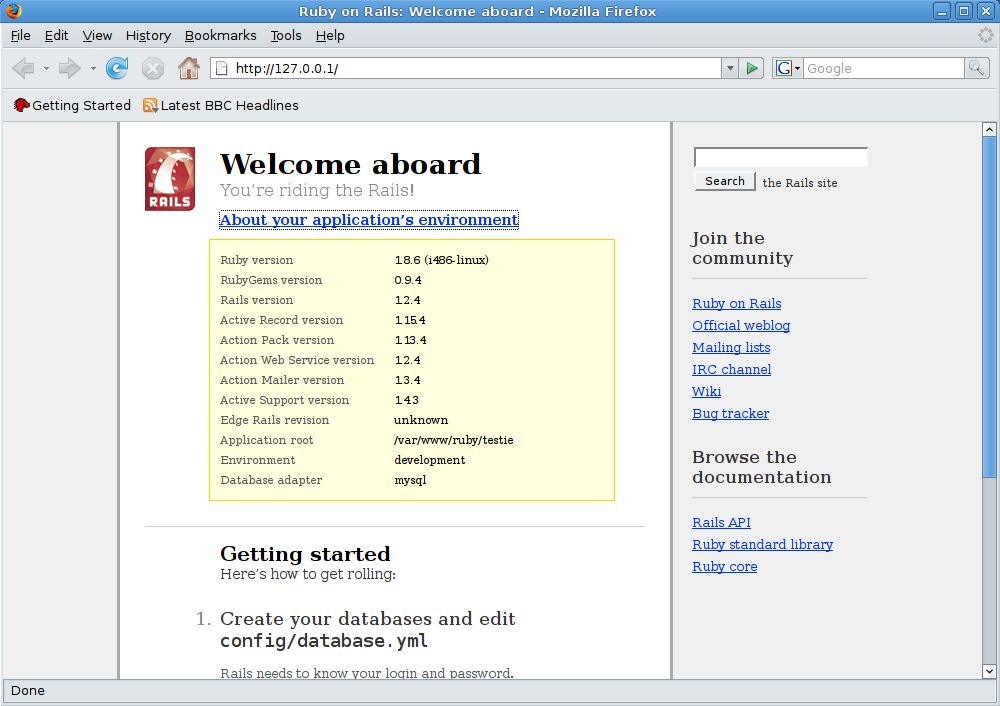
\includegraphics[width=16cm]{rubyapache.png}
\caption{Pantalla de bienvenida por defecto de rails}\label{fig:rubyapache}
\end{figure}

Existen múltiples opciones para configurar Apache de forma que soporte proyectos en Rails, un ejemplo es el proyecto \texttt{Passenger}, también llamado \texttt{mod\_rails}\footnote{Phusion Passenger - \url{http://www.modrails.com/}}, que requiere de pasos similares a los explicados anteriormente para utilizar fcgi.

\subsection{Otras consideraciones}
A lo largo de este documento no se ha tratado el tema de base de datos. Ante todas las opciones disponibles, se pueden descartar todas las que no sean libres, por un coste de licencias generalmente inalcanzable en el ámbito de este proyecto (no hay ningún tipo de subvención). De entre las opciones libres la base de datos por excelencia es MySQL\footnote{MySQL - \url{http://www.mysql.com/}}, que es considerada el compañero ideal para Ruby. A simple vista no existen requisitos extras que puedan hacer considerar alguna otra opción, por tanto se da por hecho que MySQL será el Sistema Gestor de Base de Datos de este proyecto.

\newpage
%!TEX root = /Users/simo/Documents/PFC/memoria/memoria.tex

\section{Planificación} % (fold)
\label{sec:planificacion}
El paso natural en el proceso de desarrollo de esta aplicación según las metodologías típicas sería realizar toda una etapa de diseño desde la cual se realizarían todos los diagramas correspondientes a su futura implementación. Sin embargo, y como se explicará en la sección de desarrollo, para esta aplicación se seguirá una metodología de desarrollo ágil, muy común en los entornos de desarrollo web.

Dichas metodologías defienden un desarrollo iterativo, que incluye todas las etapas (incluyendo el diseño) en cada iteración. No obstante, es necesaria una mínima planificación, especialmente para la parte de la pizarra, la cual es prácticamente independiente del resto, y por las características de Javascript hace difícil realizar un desarrollo completamente formal.

\subsection{Pizarra}
Se ha explicado con anterioridad las características de Javascript, el cual, a pesar de sus limitaciones, es orientado a objetos, y es posible programar de forma bastante modular gracias a ello. 

El código que manejará los elementos de la pizarra se distribuirá en una serie de módulos. Hay que recordar que la Pizarra está integrada en un sistema, que es la página web, que le proveerá con la información necesaria. Por ejemplo, Javascript de por si no es capaz de consultar una base de datos, pero si consultar otra página mediante Ajax, que le devuelva lo que necesita saber. Dicha página será generada por el \textbf{Sistema}, que en este caso funcionará bajo Ruby on Rails, que será el que consultará la base de datos y genere los datos con el formato adecuado para que Javascript lo pueda entender. Se puede observar la figura \ref{fig:javascript-data} a modo de ejemplo explicativo del proceso.

\begin{figure}[h]
\centering
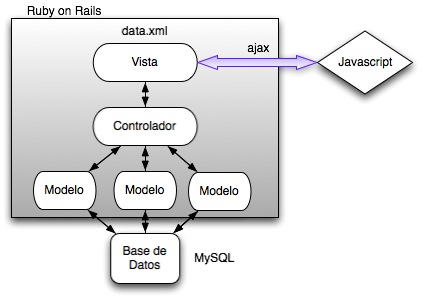
\includegraphics{javascript-data.jpg}
\caption{Esquema de la obtención de datos mediante javascript}\label{fig:javascript-data}
\end{figure}


\begin{description}
	\item[Renderizado] Aquí se agruparán las funciones que dibujen los elementos. Debe tener las funciones necesarias para poder dibujar los elementos que se soporten (líneas, polilíneas, cuadrados, círculos, etc), así como editarlos, y que sea capaz de hacerlo independientemente del navegador que se esté usando.
	\item[Dibujo] Será el módulo que controle los eventos del ponente. Debe ser capaz de entender los movimientos de ratón y teclado de forma que indique al módulo de renderizado las figuras que debe crear de forma que se experimente una sensación de dibujo interactivo. Además, debe utilizar el módulo de comunicación para informar al sistema cuándo se ha creado, editado, o eliminado algún elemento.
	\item[Comunicación] Éste módulo incluirá las funcionalidades de comunicación entre la interfaz, en javascript (recordando que javascript es incapaz de consultar bases de datos), y el sistema web. Será capaz de informar en ambas direcciones, tanto cuando el ponente ha modificado la pizarra para decírselo al sistema, como cuándo el sistema recive nuevos elementos, para comunicárselos a los espectadores.
\end{description}

Debido a las características peculiares de Javascript, se considera este enfoque como el más sencillo y eficiente para un programador con conocimientos escasos del lenguaje. El hecho de que javascript sea orientado a objetos, permite que se creen clases adecuadas para poder representar las clases del dominio, sin embargo, sigue siendo más sencillo implementar dichos controladores como una serie de funciones agrupadas en un archivo, más que hacer realmente una clase Renderizado, con subfunciones. En cualquier caso, se dará una gran importancia a intentar implementar de forma coherente con el paradigma de orientación a objetos, en la medida de lo posible acorde con las características de Javascript, y el nivel de conocimiento del lenguaje del programador. En esta fase del desarrollo es difícil definir hasta qué punto será posible.


\subsection{Sistema}

El sistema debe servir como intermediario entre todos los usuarios que participan en una pizarra, y ser capaz de realizar las funciones que Javascript, de por si solo, no es capaz. Antes de empezar a participar en alguna pizarra hay una serie de acciones que deben de ser controladas por el sistema. Dichas funcionalidades se pueden recoger en una serie de módulos, los cuales más adelante se intentarán formalizar en una estructura compatible con el paradigma Modelo-Vita-Controlador de Rails.

\begin{description}
	\item[Control de Usuarios y Grupos] Es necesario mantener un control de los usuarios y los grupos a los que se pertenece, y para ello es necesario una base de datos. Los usuarios tienen que poder registrarse y hacer las funciones típicas, como Login, edición de datos, creación de grupos, etc. Éste módulo debería ser capaz de controlar todo lo referente a usuarios y grupos según el comportamiento que se ha definido anteriormente.
	\item[Control de Pizarras] Las responsabilidades de este módulo serían las de mantener un control de las pizarras que existen, sus permisos, y su contenido. Cada pizarra tiene una serie de páginas, y cada página una serie de elementos, que deben de ser accesibles y modificables, así como poder crear o eliminar nuevos.
	\item[Comunicación con Javascript] Ésta es la funcionalidad más importante, y a falta de un nombre más apropiado, este módulo debe hacer precisamente esto, ser capaz de comunicarse con la interfaz, que se está ejecutando en el cliente, y no en el servidor. Debido a las características de Ajax y de Rails, se cree que no será posible separar formalmente estas funcionalidades, y que deberá ser incluida en los otros dos módulos.
\end{description}
\newpage



\chapter{Desarrollo: Javascript}
%!TEX root = /Users/simo/Documents/PFC/Chapter2/chapter2.tex
Según se ha establecido mediante el estudio previo, se han diferenciado dos partes muy claras. Incluso así, es posible modularizar el desarrollo de ambas partes en elementos más sencillos, que se irán uniendo con el tiempo.

Simplificando, antes de que la interfaz en Javascript pueda interactuar con el servidor, es necesario que el sistema se haya preparado y sepa como responder a las consultas. Pero para entender totalmente qué tipo de consultas deberá ser capaz de atender, se debe comprender cuál será la implementación de la interfaz, qué elementos básicos se podrán utilizar (líneas, cuadrados, texto, etc.), para así implementar las respuestas adecuadas. Y a la inversa, la interfaz necesita saber cómo serán atendidas sus respuestas para poder tratarlas correctamente.

Es necesario, por tanto, realizar una serialización del trabajo que permita entender qué se necesita de la otra parte, antes de empezar a implementarla. No solamente porque unas partes sean requisito de las otras para que funcionen, sino porque la falta de experiencia con estas dos tecnologías hace que sea necesario un proceso de comprensión previa antes de implementar completamente.

Así pues, los pasos que se han seguido son los siguientes:

\begin{enumerate}
	\item Interfaz Javascript. Implementación de los módulos de renderizado y dibujo.
	\item Sistema. Implementación de los ``modelos'' de las Pizarras y sus Elementos, con	sus controladores y vistas correspondientes, para permitir la introducción, modificación y consulta de nuevas figuras dentro de una Pizarra, y ser consultadas por la interfaz.
	\item Interfaz Javascript. Implementación del módulo de comunicación, que utiliza las vistas implementadas anteriormente de forma adecuada.
	\item Sistema. Extensión del sistema para manejar Usuarios, Grupos y Pizarras. Se añaden las vistas necesarias para que la interfaz pueda realizar consultas sobre los usuarios que participan en una Pizarra.
	\item Interfaz Javascript. Implementación del módulo de usuarios, utilizando las vistas implementadas anteriormente para poder manejar los permisos de los distintos usuarios, así como mantener a los participantes informados de quién está participando.
	\item Proceso de diseño de la web e integrado en el sistema.
	\item Funcionalidades extra: Impresión de documentos.
\end{enumerate}

\section{Javascript: Consideraciones previas}
Debido a las razones explicadas anteriormente, se deduce que Javascript es un lenguaje un tanto peculiar. Su sintaxis en la misma en todos los navegadores, pero no su DOM (Document Object Model), el cual suele cambiar sutilmente de uno a otro. Estas diferencias han hecho que tradicionalmente, saber programar en Javascript signifique conocer en profundidad dichas diferencias, y la forma en que evitarlas.

Los navegadores ``proveen'' a Javascript con dicho DOM, que no es más que una serie de objetos, a modo de librería, con los que poder consultar o modificar cualquier cosa. Por ejemplo, en cualquier momento se puede acceder a los objetos \texttt{navigator, document, window, location, screen}, etc, los cuales contienen una serie de atributos y métodos que se pueden consultar o ejecutar. Por ejemplo, el atributo \texttt{appName} del objeto \texttt{navigator} devuelve una cadena de texto con el identificador del navegador. Así, una forma sencilla de diferenciar los navegadores IE del resto sería mediante una línea como la siguiente:

\begin{verbatim}
if (navigator.appName == "Microsoft Internet Explorer") 
\end{verbatim}

Otro objeto muy importante es el \texttt{document}, a partir del cual se puede acceder y modificar todo el código html. Por ejemplo, mediante la línea siguiente se podría obtener un objeto que representaría la etiqueta \texttt{<svg id=`mainElement`>} :

\begin{verbatim}
var mainElem = document.getElementById("mainElement");
\end{verbatim}

La mayor parte del DOM es similar en todos los navegadores, haciendo las tareas típicas muy simples. Pero es en esas pequeñas diferencias en que Javascript se convierte en algo tedioso y problemático. Con el tiempo Javascript se ha ido popularizando y por lo tanto un mayor número de programadores han dedicado sus esfuerzos al lenguaje, incrementando la cantidad de documentación y librerías disponibles en proporción a dicha popularidad. Era solo cuestión de tiempo que se encontrara una solución a los problemas que se han planteado.

La solución ha aparecido en forma de librerías que permiten hacer las acciones comunes de forma unificada, encargándose ella de distinguir entre navegadores y versiones, y hacer que siempre se ejecuten los comandos apropiados. Existen diferentes librerías para esto, y en este caso se ha decidido usar jQuery. Tomando el ejemplo de querer añadir un evento a un elemento, este es el código típico que se debería ejecutar:

\begin{verbatim}
var elem = document.getElementById("body");
if(naigator.appName == "Microsoft Internet Explorer") {
   elem.attachEvent("onmousedown", doSomething);
} else {
   elem.addEvent("mousedown", false, doSomething);
}
\end{verbatim}

No solo es diferente el nombre de la función para añadir un evento, sino que en IE no se permite definir la política de bubbling, y además los nombres de los eventos son diferentes (onmousedown y mousedown).

El mismo código con jQuery incluida, quedaría así:

\begin{verbatim}
$("body").attach("mousedown",doSomething);
\end{verbatim}

Aunque aparentemente se reduzca el número de líneas, a la hora de ejecutar se tienen que hacer el mismo número de comprobaciones, quedando por tanto en un rendimiento similar, sino peor. Sin embargo, dejando todo este número de comprobaciones ``rutinarias'' de manos de una librería hace que se produzcan menos errores, pues al ser una librería pública usada por un gran número de personas, se puede asumir hayan tenido en cuenta un mayor número de factores de los que uno es capaz trabajando independientemente. Una vez más, debido a una mayor sencillez del código, es posible realizar un trabajo más limpio y libre de errores.

No solo eso, sino que es posible añadir dicha librería directamente de la página de jquery de la siguiente forma:

\begin{verbatim}
<script src="http://jquery.com/jquery-latest.js"></script>
\end{verbatim}

Puesto que un gran número de páginas usan estas librerías hoy en día, la mayoría de la gente ya habrá cargado este archivo anteriormente, reduciendo el tiempo de carga de nuestras páginas para una gran parte de nuestros visitantes, puesto que el código usando jQuery es mucho más reducido, y el cliente ya tendrá en su disco duro dicha librería.

El único problema de estas librerías es que tienen una limitación en cuanto a navegadores soportados. Lamentablemente al estar usando esta librería es posible que se reduzca el número de navegadores soportados por la aplicación, pero se considera que los beneficios de usarla sobrepasan los inconvenientes. Los navegadores soportados son más que razonables, y solamente una persona con un software extremadamente desactualizado tendría algún problema.

\newpage
%!TEX root = /Users/simo/Documents/PFC/Chapter2/chapter2.tex
\section{Javascript: Renderizado}
Se ha establecido que se utilizará VML para renderizar los elementos en navegadores Internet Explorer, y SVG en el resto, pues es la forma de conseguir llegar al mayor porcentaje de personas de forma que no necesiten instalar nada. Estas son las versiones de los navegadores que soportan dichas tecnologías:

\begin{table}[h]
	\centering
		\begin{tabular}{|c|c|}
			\hline
			Navegador & Versión \\
			\hline
			Internet Explorer & 5.0 \\
			\hline
			Mozilla Firefox & 1.5 \\
			\hline
			Safari & 3.0 \\
			\hline
			Opera & 8.0 \\
			\hline
		\end{tabular}
\end{table}

En principio podría considerarse que cualquier persona con dichos navegadores debería ser capaz de participar en una pizarra, al menos, como espectador, pero estas tecnologías no son las únicas que pueden limitar el rango de navegadores que puedan funcionar. Ya se ha comentado que la librería jQuery tiene unos requerimientos más restrictivos.

\begin{table}[h]
	\centering
		\begin{tabular}{|c|c|}
			\hline
			Navegador & Versión \\
			\hline
			Internet Explorer & 6.0 \\
			\hline
			Mozilla Firefox & 2 \\
			\hline
			Safari & 3.1 \\
			\hline
			Opera & 9.0 \\
			\hline
		\end{tabular}
\end{table}

Es imposible dar un porcentaje exacto de uso de los diferentes navegadores, pues varía dependiendo del grupo de usuarios que tiendan a visitar este tipo de webs, y por tanto, la única forma sería tener estadísticas de dicha web a lo largo de un periodo de tiempo. Sin embargo, tomando el ejemplo de una de las pocas webs que publica sus estadísticas\footnote{\url{http://www.w3schools.com/browsers/browsers_stats.asp}}, los navegadores mencionados comprenden más del 98.5\% del total.

El objetivo de este módulo es que sea capaz de realizar los dibujos de las figuras independientemente del navegador que se esté utilizando. Para ello deberán ejecutarse comandos distintos se esté en Internet Explorer (\texttt{IE} a partir de ahora) o en otro. Se pretende, por lo tanto, proveer una serie de funciones como la siguiente:

\begin{verbatim}
function createLine(here, x1, y1, x2, y2, color, thick, fill)
\end{verbatim}

Dicha función creará una línea que vaya de las coordenadas \texttt{x1,y1} a \texttt{x2,y2}, de color \texttt{color}, con un grueso \texttt{thick}, y con una transparencia del \texttt{fill}\%. Dicho elemento se anidará al elemento padre \texttt{here}.

Los elementos implementados son: línea, polilínea (trazo que pasa por una serie de puntos, como sería el resultado de un trazo a mano alzada), círculo, cuadrado, texto e imagen. Se puede encontrar la especificación de dichas funciones en el anexo, pero son generalmente suficientes para crear, modificar y eliminar satisfactoriamente todos los elementos.

\subsection{Requisitos}
Por desgracia, para que dicho módulo funcione existen una serie de requisitos. Primero, es necesario que el \texttt{HTML} sea el adecuado.

\texttt{VML} necesita dos líneas para que el navegador sepa cómo tiene que representar las directrices.
\begin{verbatim}
<html xmlns="http://www.w3.org/1999/xhtml" 
   xmlns:v="urn:schemas-microsoft-com:vml">

<style>v\:* { behavior: url(#default#VML);}</style>
\end{verbatim}

La primera línea tiene el formato típico de un documento \texttt{XML} formal. Se definen dos espacios de nombres, el princial siendo el de xhtml definido pr el \texttt{W3C}, y el segundo el de la especificación de \texttt{VML} por parte de microsoft, al cual se le añade el prefijo \texttt{v:} . Gracias a esta línea se consigue que se puedan incluir los elementos directamente en el documento, siempre y cuando empiecen por el prefijo \texttt{v:} .

La segunda línea es necesaria para que se puedan aplicar correctamente los estilos a los diferentes elementos. Dicha línea puede añadirse en cualquier punto de la cabecera (entre las etiquetas de \texttt{head}).

En cuanto a \texttt{SVG}, en cualquiera de los navegadores, es necesario que el documento sea de tipo XHTML (el código debe ser XHTML estricto, y que cuando el servidor transmita el documento, el campo \texttt{content-type} debe ser \texttt{application/xhtml+xml}. Para esto basta con cambiar la extensión del archivo a .xhtml, o modificar dicho atributo antes de ser enviado (ruby permite cambiar dicho campo, así como cualquier lenguaje de scripting como podría ser PHP). 

A diferencia de VML, SVG necesita de una etiqueta principal dentro de la cual colgarán los elementos. Debería tener una estructura como la siguiente:

\begin{verbatim}
<svg id="mainElement" xmlns="http://www.w3.org/2000/svg" 
   xmlns:xlink="http://www.w3.org/1999/xlink" 
   preserveAspectRatio="none" height="600px" width="800px">
</svg>
\end{verbatim}

El atributo id permitirá acceder fácilmente a este elemento mediante javascript. Los dos atributos xmlns son también típicos de un documento \texttt{XML}, y añaden las definiciones correspondientes a los elementos \texttt{SVG} y de \texttt{xlink}. Xlink se utiliza para referenciar elementos exteriores al documento, como podrían ser imágenes, y se explicará con más detalle en secciones posteriores. El atributo \texttt{preserveAspectRatio} ayuda a que no se deforme la imagen con posibles redimensionamientos de la ventana, y \texttt{height/width} simplemente indican el tamaño de la imagen SVG (no hay que olvidar, que al fin y al cabo estamos generando una imagen de tipo SVG).

Por último, para todo tipo de navegadores es necesario definir dos variables de Javascript, una que apunte al elemento principal del cual colgarán las etiquetas y otro que apunte al elemento exterior que servirá de referencia a la hora de calcular la posición exacta del ratón respecto al documento. En VML ambos elementos pueden ser el mismo, por lo tanto teniendo un div sería suficiente. Para SVG, sin embargo es necesario que la etiqueta SVG esté contenida dentro de una etiqueta DIV.

La razón por la cual se necesitan dos variables distintas es a causa de las diferencias en cuanto a la estructura proporcionada por el DOM. Objetos \emph{clásicos} del \texttt{HTML} como un DIV traen una serie de funciones y propiedades que el propio navegador proporciona, como son los atributos \texttt{offsetLeft} y \texttt{offsetTop}, los cuales sirven para saber la posición del ratón de forma precisa. La etiqueta SVG, sin embargo, no trae dichos atributos, con lo cual es necesario que esté ubicada dentro de un elemento estructural de HTML.

En el caso de VML esto no es necesario puesto que es posible añadir elementos VML en cualquier parte del código, y solo es necesario tener un DIV para contener todos los elementos bien ordenados y posicionados respecto al marco de lo que sería la pizarra. En SVG, al estar embediendo un documento SVG dentro de un documento XHTML, es necesario que mantenga toda su estructura típica, que es con un elemento base SVG.

\begin{figure}[h!]
\centering
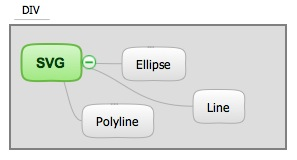
\includegraphics{divsvg.png}
\caption{Esquema del concepto de SVG dentro de un DIV}\label{fig:divsvg}
\end{figure}

Las dos variables a definir son \texttt{mainElem} y \texttt{container}.

\subsection{Implementando}
Todas las funciones de renderizado funcionan de la misma manera. Si se añadiera al código la línea siguiente:
\begin{verbatim}
  <div id="container">
    <v:line from="0,0" to="200,200">
      <v:stroke color="#000000" weight="1" opacity="0.8"/>
    </v:line>
  </div>
\end{verbatim}
se obtendría una línea que iría del punto 0,0 al 200,200 dentro del div contenedor, de color negro (\texttt{\#000000}), de 1 pixel de grosor y una opacidad del 80\%.

Lo que se pretende lograr con el módulo en javascript, es que se pueda ejecutar la línea siguiente:
\begin{verbatim}
  line = new Line(document.getElementById("mainElement"),0,0,200,200,"#000000",1,0.8);
\end{verbatim}
en cualquier momento mediante Javascript, y que automáticamente se cree ese nodo \texttt{<v:line>}. Gracias a que es posible ejecutar código javascript en cualquier evento, es posible crear una línea cuando se pulsa el ratón, e ir modificando sus coordenadas mientras se mueve. No solo eso, sinó que si se recibe alguna información, por ejemplo, mediante Ajax, es posible dibujar dinámicamente elementos a la vez que el servidor los va mandando, sin tener que recargar la página. Es posible usar, por tanto, estas funciones del motor de renderizado tanto para simular el hecho de estar dibujando (motor de dibujo), como para recibir los dibujos que realizan el resto de participantes de una pizarra (módulo de comunicaciones).

Javascript tiene todas las funciones necesarias para modificar el DOM tanto como se desee. Se ha visto que es posible obtener un elemento del código mediante el \texttt{document.getElementById}, y una vez se tiene ese objeto, existen funciones como \texttt{appendChild} para ir modificándolo.

Gracias a jQuery, y a que Javascript es un lenguaje muy relajado sintácticamente, se han podido salvar las distancias entre VML y SVG de forma bastante sencilla. Al final siempre se tiene que implementar cada función dos veces, puesto que la sintaxis de VML y SVG es diferente (hay elementos iguales, pero la sintaxis para crearlos no es la misma), pero estas funciones hacen transparente este proceso. 

\newpage
%!TEX root = /Users/simo/Documents/PFC/Chapter2/chapter2.tex
\section{Dibujo} % (fold)
\label{sec:javascript_dibujo}
La situación actual es de la disposición de una serie de funciones con las que generar gráficos vectoriales y modificarlos, funcionando en la gran mayoría de exploradores. Proceder a implementar unas herramientas de dibujo mediante esta librería es ahora posible. En esta sección no se pretende describir el proceso de creación de una herramienta de dibujo genérica, sino las peculiaridades de Javascript respecto a la forma en que trata los eventos, las diferencias entre navegadores, y la influencia de la estructura del documento (HTML y CSS).

El reto con el que uno se enfrenta inicialmente es el de conseguir capturar los eventos de ratón de forma adecuada. En los usos típicos de las herramientas deseadas, y exceptuando la introducción de texto, toda la interacción se hace mediante el ratón. Hay que recordar también el entorno en el que estas acciones se ejecutarán: habrá un marco en la página web (un elemento DIV) dentro de el cual se podrá dibujar, y una serie de elementos externos a este marco. Esto es importante puesto que es posible que los elementos exteriores interfieran de alguna forma. Dichos elementos exteriores deberán ser los siguientes:

\begin{description}
  \item[Elementos estáticos] El nombre del documento, el link de vuelta a la web \emph{normal}, así como cualquier otro elemento estático.
  \item[Barra de herramientas] Debe haber alguna forma, lo más sencilla posible, de elegir las herramientas a usar, y de configurarlas (elegir el color, grosor y transparencia). Estos elementos pueden complicar más la tarea pues deben ser dinámicos, y controlar también eventos de ratón y/o teclado.
  \item[Lista de usuarios] Esta lista deberá ser dinámica también, puesto que los usuarios podrán entrar y salir de la pizarra, y deberá informarse al resto de usuarios activos de alguna forma. No influirá con el ratón, pero si ejecutará operaciones periódicamente, y ejercerá cambios sobre el código de la página, si bien no sobre la pizarra en si.  
  \item[Selector de páginas] De la misma forma que la lista de usuarios, éste influirá poco en cuanto a eventos se refiere, pero será actualizado dinámicamente, y debe permitir flexibilidad por si el usuario no tiene permiso para cambiar de página.
\end{description}

En este momento, para dibujar, es solo necesario considerar la barra de herramientas. Más adelante, cuando se implementen más funciones, se deberá considerar cómo implementarlas, y de qué forma influencian a lo que ya se tiene.

\subsection{Barra de herramientas} % (fold)
\label{sub:barra_de_herramientas}

La opción de selección de herramientas es relativamente sencilla, puesto que solo necesita detectar cuando se clica en el elemento representativo de la herramienta y defina que esa es la herramienta activa. En javascript existen dos formas básicas de capturar eventos. La primera es utilizando el propio código HTML, con una línea como la siguiente:
\begin{verbatim}
  <div id="line-tool" onClick="setTool('line');">Línea</div>
\end{verbatim}
Todos los navegadores entienden estas definiciones, aunque no se consideran elegantes, y son bastante restrictivas por diversas razones.

Una segunda manera sería, mediante jQuery, con una línea como la siguiente (suponiendo que se quiere definir la herramienta línea al hacer click sobre el elemento con id \texttt{line-tool}):
\begin{verbatim}
  $("#line-tool").bind("click", function(){setTool('line');});
\end{verbatim}
Aunque aparentemente pueda parecer más complicada, es mucho más limpia en cuanto a que se separa lo que es el contenido de la web (HTML) con lo que es su comportamiento, de la misma forma que se separa su diseño utilizando CSS, y se considera poco elegante y práctico añadir estilos directamente en el código de los elementos.

En cuanto al problema de la configuración de las herramientas, existen múltiples y variadas soluciones. No es posible encontrar de forma nativa una manera de seleccionar un color, o de tener una barra de desplazamiento. Las únicas herramientas de las que se dispone en HTML para introducción de datos, son campos de texto o listas. Esto, aunque suficiente, es poco útil para el usuario, pues es más sencillo seleccionar un color de una paleta de colores que escribiendo su código RGB. De la misma forma, es más intuitivo usar una barra de desplazamiento para elegir el grosor o la transparencia, que escribiendo sus valores directamente. En otro tipo de herramientas sería interesante poder hacer estas cosas a mano, si se necesitara de más precisión, pero en esta aplicación es más prioritaria la agilidad de uso.

A pesar de no existir nada directamente en HTML, existen múltiples opciones que, mediante javascript, simulan estos elementos.

\subsubsection{Colores} % (fold)
\label{ssub:colores}
Para esta opción se ha decidido crear un mini-panel con ocho posibles colores, en vez de tener un selector de colores completo como los típicos de los programas de dibujo. No se cree necesario elegir una grandísima variedad de colores y con mucha precisión, sino ofrecer una pequeña cantidad de colores muy diferentes, vivos y fácilmente identificables.

\begin{figure}[h!]
\centering
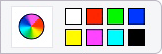
\includegraphics{color_selector.png}
\caption{Selector de colores}\label{fig:color_selector}
\end{figure}

El código para este selector es extremadamente sencillo y no consta más que de elementos sobre los que clicar para seleccionar el color, de la misma forma que se escogen herramientas.
% subsubsection colores (end) 
\subsubsection{Grosor y transparencia} % (fold)
\label{ssub:grosor_y_transparencia}
Mediante jQuery UI \footnote{jQuery UI - http://ui.jquery.com/}, una extensión a jQuery, es posible generar los llamados Sliders. Con un par de líneas de código se puede generar un Slider que permita seleccionar un valor de entre un rango, y que ejecute código personalizado al mover la manilla y al soltarla:
\begin{verbatim}
  $("#fill-dialog").slider({min: 20, max:100, startValue: 80, change: function(e,ui){
    fill = (ui.value/100);
  }, slide: function(e,ui){
    $("#fill").html(ui.value);
  }});
\end{verbatim}
Esta función crea un slider en el elemento con id \texttt{\#fill-dialog}, con posibles valores entre el 20 y el 100, puesto de forma predefinida a 80, que al cambiar actualiza el contenido del elemento con id \texttt{\#fill} (campo de texto mostrando el valor actual), y que al soltarse actualiza la variable \texttt{fill} con el valor seleccionado.

\begin{figure}[h!]
\centering

\includegraphics{fill_selector.png}
\caption{Slider selector de relleno (transparencia)}\label{fig:fill_selector}
\end{figure}

% subsubsection grosor_y_transparencia (end)


% subsection barra_de_herramientas (end)

\subsection{Eventos de ratón} % (fold)
\label{sub:eventos_de_raton}

Los tres eventos básicos de un ratón son los de pulsar un botón (\texttt{mousedown}), moverse (\texttt{mousemove}) y soltar el botón (\texttt{mouseup}). Los tres son necesarios, puesto que son, en ese orden, cuando se empieza a dibujar un elemento, cuando se va modificando, y cuando finalmente se \emph{suelta}, quedando gravado definitivamente hasta que es borrado (a excepción del texto, que es un tanto más peculiar, y se explica en otro apartado).

El que solo se quiera poder dibujar dentro del marco seleccionado para ello, hace que se planteen una serie de problemas.

\begin{itemize}
  \item Cuando se empieza a dibujar dentro del marco, pero se mueve el ratón fuera de él.
  \item Cuando se suelta el botón fuera del marco.
  \item O peor aún, cuando se suelta el botón fuera de la ventana.
\end{itemize}

\subsubsection{¿Cómo funcionan los eventos en Javascript?} % (fold)
\label{ssub:como_funcionan_los_eventos}

En Javascript es posible capturar eventos en cualquier elemento, y siempre sucederá de forma jerárquica según la visibilidad que se tiene de los distintos elementos. Es decir, si se tiene un trozo de código como el siguiente:
\begin{verbatim}
  <div>
    <p>Hola <a id="albert-link" href="/users/albert">Albert</a>, qué tal estás?</p>
  </div>
\end{verbatim}

y se hace click en la palabra Albert, saltará un evento en el elemento \texttt{a}, cuando acabe de hacer lo que sea que debe hacer, y pasará a ejecutar el evento del elemento \texttt{p}, seguirá con el del \texttt{div}, y acabará con el del elemento \texttt{body}, que en cada documento HTML es el contenedor de todo lo que se ve en pantalla. Por tanto, si se quisiera capturar cualquier movimiento de ratón en la pantalla, se deberían capturar los eventos \texttt{mousemove} del elemento \texttt{body}.

Por otro lado, el ejemplo anterior tiene un problema, y es que el evento \texttt{click} de todo elemento \texttt{a} lo que hace es mandar al usuario a la página que éste linca. En caso de querer, por ejemplo, en vez de mandar al usuario a la página con los detalles personales de Albert, que está en \texttt{/users/albert}, si no que queremos hacerlo más dinámico y mostrarlo directamente mediante Javascript, se debería capturar el evento click de dicho elemento, y realizar lo necesario (una llamada por ajax, creación o modificación de otro elemento para mostrar la información, etc). Pero el comportamiento de los eventos en Javascript, por defecto, al acabar de atender el evento capturado por el usuario, sigue ejecutando el comportamiento normal de dicho elemento (ir a la página enlazada), a menos que la función ejecutada devuelva un valor falso.

Es decir, el código javascript debería ser semejante al siguiente:
\begin{verbatim}
  $("#albert-link").bind("click",function(){
    // Obtener información y mostrarla dinámicamente
    . . .
    return false;
  });
\end{verbatim}

Esto es considerado una buena técnica puesto que en caso de estar ante un usuario sin soporte para Javascript, el sistema mostrará la información de todas maneras, aunque no de una forma tan dinámica. En el caso que interesa a este proyecto, hay que comprender este comportamiento para que, por ejemplo, se pueda seguir dibujando aun estando fuera del marco, o para tener varias cosas que estén encima del marco, poder trabajar con ellas mediante eventos, y que éstos no influyan al proceso de dibujo.

% subsubsection como_funcionan_los_eventos (end)

\subsubsection{¿Cómo capturarlos?} % (fold)
\label{ssub:como_capturarlos}

En este caso, por el comportamiento que se le quiere dar a la aplicación, es necesario estar siempre al tanto de los siguientes eventos:
\begin{itemize}
  \item Cuando se pulsa un botón del ratón dentro del marco. Si se pulsa el ratón fuera del marco, no debe afectar al dibujo, más que en el caso de las herramientas o el selector de páginas, pero estos trabajan de forma independiente.
  \item Se debe saber en todo momento cuándo se está moviendo el ratón, y cuándo se suelta el botón, debido a los casos explicados anteriormente, si va dibujando hasta soltar el ratón fuera del marco, o de la ventana. Si se ignoraran los eventos fuera del marco, se producirían comportamientos incómodos, como que se deje de mover una línea por rozar un borde, o que, al no enterarse de que se ha soltado el botón, se siga dibujando aún cuando no se está pulsando.
\end{itemize}

Sabiendo, como se ha comentado antes, que siempre se tendrá un elemento con id \texttt{\#container}, que será el \texttt{marco}, el código para capturar los eventos es el siguiente:

\begin{verbatim}
  $(document).ready(function(){
    $(container).bind("mousedown", mouseDown);
    $("body").bind("mousemove", mouseMove);
    $("body").bind("mouseup", mouseUp);
  });
\end{verbatim}

En este caso, en vez de implementar las tres funciones directamente, se pasan como parámetro. Puesto que Javascript entiende las funciones también como objetos, es posible definirlas con anterioridad de la misma forma que se definiría una variable, para luego usarla como parámetro. jQuery automáticamente pasa a estas funciones la \textbf{variable de evento}, que es un descriptor del entorno en que ha sucedido el evento. Cosas como la posición del ratón, el elemento al que se estaba apuntando, qué botón se ha pulsado, se pueden consultar en este objeto.

% subsubsection _cómo_capturarlos_ (end)

\subsubsection{¿Dónde está el ratón?} % (fold)
\label{ssub:donde_esta_el_raton}

No hay que olvidar, que lo que se está haciendo es, en cierta medida, \emph{incrustar} un elemento SVG, o un conjunto de elementos VML, dentro de otro elemento DIV. A la hora de crear elementos, por tanto, es necesario especificar las posiciones como pixels respecto del inicio del marco. Mediante jQuery es posible obtener la posición absoluta del ratón, respecto del total de la ventana del navegador, pero para este caso es necesario algo más preciso, que tenga en cuenta también la posición del DIV, y o si se ha hecho scroll o no.

Los atributos que se pueden consultar mediante la \textbf{variable de estado} (\texttt{event} a partir de ahora) del evento, y el resto del DOM, y que son útiles para posicionar elementos, son las siguientes.

\begin{description}
  \item[\texttt{event.clientX} y \texttt{event.clientY}] Estos atributos devuelven la posición del ratón respecto a lo que ahora se ve en el navegador. Esto quiere decir, aunque se haya hecho scroll, si se clica en la esquina superior izquierda, ambos valdrán 0.
  \item[\texttt{container.offsetLeft} y \texttt{container.offsetTop}] Recordando que \texttt{container} es el DIV contenedor dentro del cual se anidarán los elementos, estos dos atributos devuelven su posición respecto a los bordes absolutos de la página, ignorando si se ha hecho scroll o no.
  \item[\texttt{document.body.scrollLeft document.body.scrollTop window.pageXOffset window.pageYOffset}] Este es un claro ejemplo de las diferencias comentadas entre el DOM ofrecido por diferentes navegadores, y que generalmente jQuery ayudaría a resolver. Los dos primeros funcionarían en \texttt{IE}, y devuelven la cantidad de pixels que se ha hecho scroll, tanto lateral como verticalmente, y los segundos son sus equivalentes para todo el resto de navegadores.
\end{description}


\begin{figure}[h!]
\centering
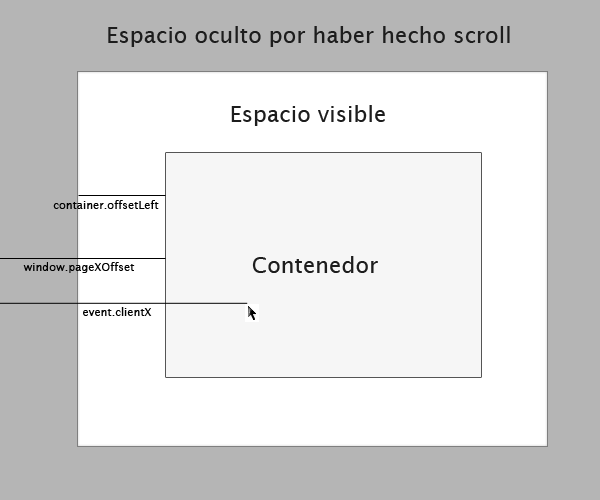
\includegraphics[width=\textwidth]{mouse_pointer.png}
\caption{Esquema de distancias de los distintos elementos}\label{fig:mouse_pointer}
\end{figure}

La figura \ref{fig:mouse_pointer} muestra un pequeño esquema de estas distancias. Mediante estos tres tipos atributos es posible averiguar la posición del ratón respecto al DIV contenedor, sea cual sea la situación de la página, con estas instrucciones.

\begin{verbatim}
//IE
x = e.clientX - container.offsetLeft + document.body.scrollLeft;
y = e.clientY - container.offsetTop + document.body.scrollTop;
//RESTO
x = e.clientX - container.offsetLeft + window.pageXOffset;
y = e.clientY - container.offsetTop + window.pageYOffset;
\end{verbatim}

Con estos conocimientos ya es posible programar las herramientas de línea, trazo de lápiz, elipse y caja, que son la base de lo que este proyecto pretendía. El resto del trabajo necesario para programar estas herramientas es de puesta en práctica de estos apartados, y no se considera importante destacar nada más. El código de la implementación se puede encontrar en el anexo.

% subsubsection donde_esta_el_raton (end)

% subsection eventos_de_ratón (end)

\subsection{Introducción de texto} % (fold)
\label{sub:introduccion_de_texto}

El método tradicional para introducir texto en páginas web, es mediante los elementos de formulario \texttt{input} de tipo \texttt{text} o los llamados \texttt{textarea}. Para esta situación el más adecuado será el \texttt{textarea} puesto que el otro es simplemente una línea, y los \texttt{textarea} se pueden redimensionar a voluntad.

El efecto que se quiere lograr es el de crear un pequeño recuadro donde escribir, y al hacer click fuera o pulsar tabulador, este texto pase a formar parte del documento. Existe un requisito importante, y es que la posición del texto mientras se escribe, y cuando se introduzca \emph{definitivamente}, debe ser la misma, para así no confundir al usuario.

Este proceso difiere del resto de herramientas por necesitar de dos pasos distintos, uno para crear un \texttt{textarea} en alguna posición, y otro para acabar agregándolo finalmente.

\subsubsection{Generación de un textarea} % (fold)
\label{ssub:generacion_de_un_textarea}
En este caso, la creación del elemento no será en el evento \texttt{mousedown}, puesto que los usuarios están acostumbrados que las cosas suceden al soltar el botón del ratón, no al pulsarlo. Al detectar un evento de tipo \texttt{mouseup} con la herramienta de texto seleccionada, y siempre y cuando se haya clicado antes dentro del contenedor, se crea dinámicamente este textarea, posicionado mediante CSS con origen en la posición del ratón.

% subsubsection generación_de_un_textarea (end)

\subsubsection{Introducción del texto} % (fold)
\label{ssub:introduccion_del_texto}
Para poder averiguar cuando el usuario quiere dejar de escribir e introducir el texto en el documento, hay que simular de alguna manera las distintas posibilidades por las que un usuario puede pretender hacer esto. Lo más intuitivo es que esto suceda cuando el elemento pierda el \texttt{focus}, es decir, cuando se clique fuera o se pulse tabulador. La forma de asegurarse que esto sucede es capturando los eventos \texttt{change} y \texttt{blur}, además de mediante los eventos que ya se capturan de mousedown y mouseup.

Al detectar este suceso, se genera un nuevo DIV, que estará anidado dentro de del contenedor igual que el resto de elementos, y posicionado mediante CSS en el mismo lugar en el que estaba el \texttt{textarea}, con la misma fuente, tamaño y color.


% subsubsection introducción_del_texto (end)

% subsection introducción_de_texto (end)

\subsection{Goma de borrar} % (fold)
\label{sub:goma_de_borrar}

Existen dos vertientes diferentes a la hora de plantear la goma de borrar. La funcionalidad típica a la que se está acostumbrado en los programas de dibujo, es a la de una goma que, de forma inversa a lo que sería el lápiz, borra solamente el trozo por el que se pasa por encima. Esta vertiente, por el tipo de datos con los que se está trabajando, sería extremadamente difícil de implementar, pues al pasar por en medio de un elemento, se debería detectar en qué punto ha pasado, y dividir los elementos en múltiples trazos (si son líneas o trazos de lápiz), o prácticamente imposible de representar si se tratara de una caja o una elipse.

La otra vertiente, más usada en los programas de pizarra compartida por la sencillez, tanto para el programador, como para el usuario, es la una goma de borrar que no elimina solo aquellas zonas por las que pasa, sino que elimina el elemento entero. Situándose en la posición del usuario que está utilizando esta pizarra para acompañar sus explicaciones, la situación clásica es la de estar resaltando distintos elementos de la página, que luego querrá eliminar para seguir su explicación. Tener la facilidad de clicar en el elemento, y que este desaparezca por completo, sería muy práctico, y posiblemente la mejor solución.

Existen múltiples formas de enfocar este problema, puesto que es posible capturar eventos del ratón en cualquiera de los elementos que se generan, no solamente en el contenedor. Sin embargo, se considera que esto es excesivamente complejo, y que gracias al atributo \texttt{target} de la \textbf{variable de estado} del evento, es posible solucionar todos los problemas con los eventos que ya se capturaban con anterioridad.

Suponiendo que se tiene la herramienta de goma de borrar seleccionada, y que se quiere borrar algo que está en un punto donde coincide, por ejemplo, un círculo y una línea. El círculo se ha dibujado después de la línea, por lo tanto está por encima, así que lo más lógico es que se borrara primero. Al hacer click, el evento se generará en el elemento círculo, pues es el que está visible en ese momento, pero tal y como se ha explicado en la sección \textbf{¿Cómo capturarlos? }\ref{ssub:como_capturarlos}, este evento irá saltando de superior al inferior, llegando, en efecto, a los eventos que se capturan en el contenedor o en la etiqueta \texttt{body}.

Una vez más, mediante la \texttt{variable de estado} es muy fácil saber cuál fue el objeto que generó el evento originalmente, a pesar de que en ese momento se esté tratando el evento de un elemento \emph{inferior}. Y una vez más, existe un conflicto entre los atributos generados por \texttt{IE}, y los atributos generados por el resto de navegadores.

\begin{verbatim}
// IE
event.srcElement
// SVG
event.target
\end{verbatim}

% subsection goma_de_borrar (end)

% section javascript_dibujo (end)
\newpage
%!TEX root = /Users/simo/Documents/PFC/Chapter2/chapter2.tex
\section{Comunicación} % (fold)
\label{sec:javascript_comunicacion}
En estos momentos ya es posible renderizar gráficos vectoriales, así como poder dibujarlos de forma interactiva. Es, a efectos prácticos, una \textbf{Pizarra Web}, faltando solo hacerla compartida. Para conseguir esto se han de conseguir dos funcionalidades básicas:

\begin{description}
  \item[Persistencia de los elementos] Es necesario que al crear y eliminar elementos, estos se refleje en una base de datos de fondo, para que en un futuro, estos elementos siguen ahí, y para que el resto de la gente pueda obtener esos elementos.
  \item[Comunicación entre usuarios] Es decir, que los elementos generados por un usuario sean vistos por el otro, de forma automática.
\end{description}

La naturaleza de la web hace esto realmente complicado. El flujo interacción entre un úsuario y una página web es el siguiente:

\begin{figure}[h!]
\centering
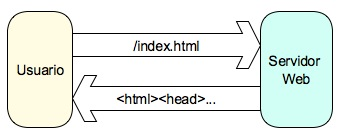
\includegraphics{navigation.png}
\caption{Interacción usuario - servidor}\label{fig:navigation}
\end{figure}

Es un una interacción totalmente pasiva por parte del servidor, el cual solo contesta cuando y si se le solicita un documento. No solo eso, sino que típicamente, la forma de navegar por páginas webs es de ir recargando cada página individualmente. Para este proyecto se necesita algo más, pues la interacción entre el usuario y el servidor tiene que ser totalmente transparente, y por supuesto la página no debe de recargarse cada vez que suceda algún cambio.

En el año 2002, y con el navegador Internet Explorer 5 \footnote{http://es.wikipedia.org/wiki/XMLHttpRequest}, se introdujo la interfaz \texttt{XMLHttpRequest}, que permite abrir conexiones  HTTP con el servidor de forma dinámica mediante Javascript, de forma transparente al usuario, puesto que no necesita recargar la página. Gracias a esto, es posible establecer un flujo de información entre el usuario y el servidor, con el que no solamente transmitir los cambios que dicho usuario haga al documento, sino que permita recibir información de lo que el resto de gente hace.


Las conexiones \texttt{XMLHttpRequest} tienen las mismas características que cualquier otra conexión abierta por un navegador de forma tradicional, con las únicas limitaciones de no poder enviar o recibir archivos de caracter binario. Eso quiere decir que, por ejemplo, es posible pasar parámetros. La diferencia, sin embargo, es que para este tipo de peticiones, no es nada útil que el servidor conteste con documentos que sean páginas web típicas, sino que es necesario que la información sea devuelta en algún formato fácil de entender por un lenguaje de scripting como Javascript. Habitualmente se usa XML, de ahí el nombre de la interfaz, pues es una sintaxis muy adecuada a este tipo de usos, pero es posible recibir cualquier tipo de texto, y de hecho, existen mejores alternativas cuando dicho resultado se va a usar con Javascript. En aplicaciones más modernas se utiliza JSON \footnote{http://es.wikipedia.org/wiki/JSON}, que es básicamente la misma sintaxis utilizada en Javascript para generar objetos (Arrays y Hashes).

\begin{verbatim}
  {
    "page":1,
    "objets": [{"type":"line","x1":10,"x2":20,"y1":0,"y2":5},
               {"type":"circle","x":20,"y":20,"radius":15}]
  }
\end{verbatim}

Ese mismo trozo de código, si se escribiera dentro de una pieza de código Javascript, generaría un Hash con dos atributos, \texttt{page} y \texttt{objects}, y object sería un Array con dos elementos, que a su vez son Hashes. Teniendo ese trozo de texto, en la variable \texttt{response} por ejemplo, que se ha consultado mediante XMLHttpRequest, solo hay que ejecutar la función \texttt{eval} sobre \texttt{response} para generar el objeto correspondiente.

Como era de esperar, la forma de realizar consultas mediante XMLHttpRequest difiere de un navegador a otro, por eso es muy útil utilizar alguna librería, en este caso jQuery, que lo hace tan fácil como usar la función \texttt{get(url)} para consultar una página mediante \texttt{GET}, o \texttt{post(url)} para hacerlo mediante \texttt{POST}.

\begin{verbatim}
  response = $.get("/list_of_elements.json");
  object = eval(response);
  alert(object.page);
\end{verbatim}

Suponiendo que el documento \texttt{list\_of\_elements.json} contiene el trozo de JSON anterior, al realizar un \texttt{alert(object.page)}, se mostrará el valor \textbf{1}.

De la misma forma, se puede utilizar la versión más completa de las funciones para poder enviar información:

\begin{verbatim}
  $.ajax({
    type: "POST",
    url: "/save_circle",
    data: {x: 1, y: 2, radius: 20}
  });
\end{verbatim} 

este comando crearía una solicitud HTTP como la que se genera cuando se rellena un formulario, mandándola mediante POST, con los atributos especificados en data. Lógicamente es necesario un sistema que sea capaz de entender todas estas solicitudes, pero por ahora este capítulo se centrará en como el Javascript tratará todas las comunicaciones necesarios con el servidor, suponiendo siempre que existe el sistema que actuará de forma adecuada.

\newpage
\subsection{Crear y destruir elementos} % (fold)
\label{ssub:crear_y_destruir_elementos}

Esta parte es la más sencilla, puesto que solo es necesario comunicar al servidor de los cambios realizados por el usuario en concreto. En todos los casos está muy claro cuando se crea un elemento, y cuando se elimina, por tanto, ese será el momento de comunicarlo. 

El primer problemaes decidir de qué forma se va a representar un elemento. Recordando que cada elemento tiene atributos diferentes, y que todo ha de acabar siendo almacenado en una base de datos relacional, es posible que todo pueda llegar a complicarse. Lo más sencillo en este caso sería que todos los elementos, sean del tipo que sean, pudieran ser guardados en una misma tabla de una base de datos, y que por tanto, tubieran los mismos atributos.

Puesto que siempre que se consulten datos al servidor, éste los comunicará en forma de JSON, se ha creído adecuado que ocurra el mismo proceso en sentido inverso. La forma de que todos los objetos puedan estar en la misma tabla, es codificándolos de alguna manera de forma que puedan representarse mediante una cadena de texto. De la misma forma que, con una cadena de texto en formato JSON es posible generar un objeto en Javascript, es posible realizar el proceso opuesto. Suponiendo la existencia de una función \texttt{toJSON(object)} que devuelva un string representativo del objeto, el proceso para comunicar al servidor un nuevo elemento, podría ser el siguiente:

\begin{verbatim}
  function save(it){
  	var text = toJSON(it);
  	$.ajax({
  		url: "/add_element",
  		data: {attr: text}
  	});
  }
\end{verbatim}

Ésta es una versión simplificada de la función que se ha acabado usando en realidad, pero ya sirve para ver el proceso que se ha seguido. Es necesario añadir una serie de mejoras, que se comentan a continuación.

¿Cómo sabe el sistema a qué documento pertenece este elemento? Es necesario enviar información para que se sepa a qué documento corresponde este elemento. Puesto que habrá una base de datos de fondo, es posible suponer que siempre habrá un identificador para documento, y que es conocido de alguna manera por el javascript, pues se habrá definido al cargar la página.

\begin{verbatim}
  function save(it){
  	var text = toJSON(it);
  	$.ajax({
  		url: "/add_element",
  		data: {attr: text, :doc: docId}
  	});
  }
\end{verbatim}

La parte de crear elemento se puede considerar como resuelta. En cuanto eliminar objetos, es necesario saber algo más. ¿Cómo se le comunica al sistema qué elemento se ha eliminado? De la misma forma, es posible suponer que en la base de datos, estos objetos tendrán asignado un identificador como clave primaria. Este identificador se genera al crear dicho elemento, por lo tanto no es posible saberlo hasta que no se ha comunicado al servidor. La solución para esto es modificar la función de guardado de elementos, haciendo que el servidor conteste a la consulta que agrega un elemento, con el id generado para dicho elemento. Aunque una consulta se utilice para transmitir información, el servidor siempre debe contestar algo, por lo tanto es posible aprovechar estos datos:

\begin{verbatim}
  function save(it){
  	var text = toJSON(it);
  	$.ajax({
  	  url: "/add_element",
  	  data: {attr: text, :doc: docId},
  	  success: function(ret){
  	    it.element.id=ret;
  	  }
  	});
  }
\end{verbatim}

Este cambio agrega código personalizado al evento success de esta consulta XMLHttpRequest. jQuery lanza eventos en diferentes puntos de las consultas para que el programador pueda ejecutar distintas acciones en los distintos puntos de la consulta. Los eventos generados son \texttt{beforeSend, complete, success} y \texttt{error}, todos ellos suficientemente descriptivos.

En este caso, cuando la consulta finaliza y es satisfactoria, y suponiendo que el servidor ha contestado simplemente con el id del elemento creado, se coge el objeto que se había guardado, y se modifica añadiéndole un campo id con dicho valor. De esta forma, los elementos representados en pantalla tienen el id correspondiente a su equivalente de la base de datos, y permiten, por tanto, simplificar la función de borrado a un simple:

\begin{verbatim}
  //IE
  $.get("/remove_element/" + event.srcElement.id);
  //RESTO
  $.get("/remove_element/" + event.target.id);
\end{verbatim}

utilizando, como ya se había comentado anteriormente, los atributos \texttt{srcElement} y \texttt{target} de la \textbf{variable de estado}, para saber con qué elementos se estaba tratando.

% subsubsection crear_y_destruir_elementos (end)
\newpage
\subsection{Sincronización entre usuarios} % (fold)
\label{ssub:sincronizacion_entre_usuarios}

Uno de los mayores retos a los que se enfrenta esta aplicación, es mantener a todos los usuarios sincronizados. Hasta este momento es posible mantener al servidor informado de la creación y eliminación de elementos, pero no es posible informar al resto de usuarios de dichas acciones. En el caso de aplicaciónes típicas, con un paradigma cliente-servidor en que el servidor pudiera iniciar transferencias de información, lo lógico sería que cuando hubiera algún cambio, el servidor informara al resto de clientes de los cambios.

Sin embargo, en el caso de una página web, esto no es posible. No hay ninguna posibilidad de que el servidor establezca una conexión con el usuario por iniciativa propia, y por tanto la única solución restante es realizar consultas periódicas en busca de nuevos cambios. El tiempo entre consulta y consulta, así como la latencia entre el servidor y el cliente, son los factores que definen el tiempo entre que se realiza un cambio y el momento en que el resto de usuarios es consciente de ello.

Teniendo en cuenta que la latencia es un parámetro incontrolable, la única posibilidad para mejorar los tiempos es cambiar el tiempo entre una consulta y otra. Existen dos estrategias posibles para esto, ambas perfectamente viables, aunque adecuadas para diferentes necesidades.

\subsubsection{Realizar peticiones cada periodo de tiempo fijo} % (fold)
\label{ssub:nunca_tener_más_de_una_petición_pendiente}
El enfoque más directo y más logico en un primer acercamiento al problema, es ir lanzando peticiones periódicamente, sin importar que peticiones anteriores hayan sido contestadas ya o no. Suponiendo una latencia de unos 200ms entre servidor y usuario, el tiempo de estabilidad $t_e$ será de $ 2t_l < t_e > 2t_l + t_r$ con $t_l$ siendo la latencia y $t_r$ el tiempo entre peticiones. Este enfoque permite personalizar al máximo el comportamiento de la aplicación, pudiendo tener mejores tiempos si se dispone de recursos suficientes, o empeorándolos en caso contrario.

Sin embargo, este enfoque produce una serie de problemas asociados al hecho de tener conexiones simultáneas pendientes. Debido a que la latencia no es un número fijo, y por tanto es posible completar peticiones en orden distinto al que se han generado, se debería realizar todo un control de paquetes semejante al realizado por TCP en las redes de datos, para permitir un comportamiento adecuado de la aplicación.

\begin{quotation}
  Un elemento es creado en momento $0$ por el usuario $u1$. El servidor, debido a la latencia, recibe notificación del cambio en el momento $10$. Mientras tanto, el usuario $u2$, ha ido mandando peticiones cada unidad de tiempo, pero debido a la inestabilidad de la red, recibe primero el resultado de una petición que llegó al servidor en el momento $11$, antes que otra que había llegado al servidor en el momento $9$. Debido a ello, primero recibe notificación de borrar el elemento, puesto que ya no está, y después la segunda notificación le informa de que aún sigue ahí.
\end{quotation}

Este es solo el primero de varios problemas posible, sin tener en cuenta que varios usuarios pueden agregar o eliminar elementos al mismo tiempo, cambiar de página, o que el servidor se caiga y se deje de recibir contestaciones. No es, ni mucho menos, una tarea imposible de realizar, pero si requiere de un grado de control extra.

% subsubsection nunca_tener_más_de_una_petición_pendiente (end)

\subsubsection{Una petición a la vez} % (fold)
\label{ssub:una_peticion_a_la_vez}
Otro enfoque posible es el de ir realizando peticiones contínuas, pero siempre una detrás de otra. Es decir, generando la petición, procesando la respuesta, y generando una petición inmediatamente después. Con este planteamiento es posible ignorar la mayoría de problemas de sincronización comentados, y permitirá una menor carga por parte tanto del servidor como del navegador del usuario. El tiempo de estabilidad en este caso, sería de $ 2t_l < t_e > 4t_l$ . De nuevo, tomando una latencia media de 200ms, se baraja un $t_e$ de casi un segundo.

Comparando con la estrategia anterior, sin embargo, se puede observar que esta diferencia no es tan acentuada. Un planteamento realista no contemplaría más de cuatro o cinco peticiones por segundo, en cuyo caso se estaría hablando de nuevo, de un $t_r$ de 200ms, con lo cual se estaría en un $t_e$ entre 400ms y 600ms (500ms de media). Comparado con esta segunda estrategia, en la cual se maneja un $t_e$ de entre 400 y 800ms (600ms de media), solo se obtendría un beneficio de unos 100ms de media, además de reducir de $5$ peticiones por segundo a $2,5$.

Con una diferencia tan pequeña, no se considera necesario el esfuerzo necesario para mantener un sistema con el primer enfoque, y que el segundo, siendo más sencillo y robusto, permitirá una mayor fiabilidad del código.

% subsubsection una_peticion_a_la_vez (end)

% subsubsection sincronización_entre_usuarios (end)

% section javascript_comunicacion (end)



\chapter{Desarrollo: Ruby on Rails}
%!TEX root = /Users/simo/Documents/PFC/memoria/memoria.tex
Se dispone en estos momentos de un motor completo en Javascript que permitiría todo el proceso necesario para los objetivos de este proyecto. Éste, sin embargo, necesita de un fondo que le aporte todo lo que html estático y javascript no es capaz de hacer, como por ejemplo, tratar con la base de datos. Por las razones comentadas en el primer capítulo, se ha considerado que Ruby on Rails sería la solución para implementar este fondo, y en este capítulo se comenta el proceso seguido, resaltando en cada caso las diferencias de utilizar Ruby on Rails frente a soluciones más clásicas como PHP o ASP.

\section{Consideraciones previas} % (fold)
\label{sec:ruby_on_rails_consideraciones_previas}
Antes de nada, para entender como funciona Ruby on Rails, hay que aclarar ciertos conceptos. Primero, el lenguaje en que se está programando es Ruby. Éste es un lenguaje interpretado, que al igual que lenguajes de scripting típicos como Perl, PHP o Python, se compilan dinámicamente a la hora de la ejecución. De hecho, existen implementaciones de interpretadores de Ruby en varios lenguajes, siendo la implementada en C la \emph{oficial}, pero existiendo otras tan dispares como jRuby, una implementación en Java que permite utilizar cualquier librería de Java.

Ruby es un lenguaje de alto nivel, con una sintaxis que hace que sea muy fácil de entender para gente que no la conoce. Por ejemplo:

\begin{verbatim}
100.times do 
  print "No hablaré en clase".upcase
end  
\end{verbatim}

La popularidad de Ruby se ha incrementado con el éxito de Ruby on Rails, y ha hecho que se puedan encontrar librerías para prácticamente cualquier cosa. La sencillez del código lo hacen muy adecuado para el mundo del desarrollo web, donde se prioriza la agilidad de desarrollo, antes que una gran eficiencia. Existen múltiples técnicas de cacheo que hacen que el procesado necesario por el lenguaje de scripting sea mínimo, relegando todo el trabajo al servidor web (Apache, por ejemplo), y a unas consultas a la base de datos bien eficientes. Por tanto, lenguajes de más bajo nivel que podrían aportar una mayor eficiencia del código no se consideran adecuados por requerir de un proceso de desarrollo más largo y costoso, para unas ganancias relativamente mínimas. El uso de este tipo de lenguajes se relega a partes muy pequeñas y precisas, normalmente en los culos de botella donde puedan ser útiles. Se considera más beneficioso poder desarrollar más, de forma más sencilla para así evitar bugs indeseables, y utilizar dichas técnicas de cacheo y de gestión de base de datos para lograr la eficiencia.

Rails es un Framework escrito en ruby que permite un desarrollo web ágil y sencillo. Se basa en hacer fácil el trabajo del programador, y en su famoso \emph{Convention over configuration} (convención antes que configuración). Debido a que la mayoría del tiempo, el desarrollo de webs es un proceso repetitivo, es posible establecer una serie de patrones que asumir, y solo modificar en los casos especiales en que \emph{lo normal} no es suficiente.

Está basado en una arquitectura MVC (Modelo Vista Controlador), permitiendo aplicar el patrón en 3 capas estudiado las diversas asignaturas de Ingeniería del Software, así como la mayoría de buenas prácticas, hasta ahora mayoritariamente difíciles de aplicar en el mundo del desarrollo web.

Rails, gracias a la sencillez de Ruby, promueve la práctica del desarrollo ágil de software (Agile software development), una metodología de desarrollo que se basa en aligerar el proceso de desarrollo, alejarse de metodologias \emph{burocráticas}, centrándose en conseguir software de alta calidad de forma muy rápida. Estas características son muy apreciadas en el mundo del desarrollo web, puesto que como ya se ha comentado, la eficiencia suele ser secundaria, y los procesos, al ser repetitivos en su mayoría, hacen de otras metodologías demasiado pesadas y lentas.

A lo largo de este capítulo se irán remarcando los puntos por los cuales Ruby es tan adecuado al desarrollo web, porqué Rails permite un desarrollo más ágil, y porqué una metodología basada en la escasez de documentación y planificación es posible, y de hecho, beneficiosa, en el contexto de este proyecto (y en el de otros similares de desarrollo de webs). 

% section ruby_on_rails_consideraciones_previas (end)

\newpage
%!TEX root = /Users/simo/Documents/PFC/Chapter3/chapter3.tex
\section{Primer ciclo} % (fold)
\label{sec:primer_ciclo}
La metodología de desarrollo ágil defiende un desarrollo iterativo, por ciclos perqueños que generen de forma rápida ciertas funcionalidades. Cada ciclo amplica funcionalidades hasta que al final estén todas incluidas. Cada ciclo debe ser completo, con sus fases de análisis de requisitos, diseño, implementación y revisión. La fase de documentación tiene como resultado este capítulo.

En este primer ciclo, se pretende obtener todas las funcionalidades necesarias para poder crear y editar documentos.

\subsection{Análisis de requisitos} % (fold)
\label{sub:análisis_de_requisitos}

Gracias a que se ha tratado la implementación del Javascript de forma previa a este ciclo, se conocen ya los requisitos básicos necesarios para poder utilizar el motor de dibujo. De firna detallada, las funcionalidades requeridas para este ciclo son las siguientes:

\begin{itemize}
  \item Poder crear, editar y borrar documentos, dándoles un título, una descripción y asignándole una cantidad de páginas fija, mediante interacción normal por HTML.
  \item Tener soporte para documentos, páginas y los elementos contenidas en ellas, de forma que el motor de comunicación en Javascript pueda comunicarse con la aplicación para editar las pizarras.
\end{itemize}

% subsection análisis_de_requisitos (end)

\subsection{Diseño} % (fold)
\label{sub:diseño}

El primer paso natural a la hora de planear un ciclo en Ruby on Rails es planeando la estructura de la aplicación en cuanto a modelos y controladores se refiere. Los modelos serán necesarios para poder guardar los datos en la base de datos, y deben estar relacionados adecuadamente de forma que sea fácil y directo acceder a datos de modelos \emph{cercanos}. También es importante considerar los controladores en los que agrupar las funciones. Sería posible implementar la aplicación entera en un controlador enorme, pero obviamente esto no sería práctico ni productivo.

\subsubsection{Modelos} % (fold)
\label{ssub:modelos}

El diagrama de clases es extremadamente sencillo en este ciclo. Solamente son necesarias tres clases, una para representar el documento, otra para las páginas y otra para los elementos. Durante la discusión sobre la implementación del javascript ya se discutió que la descripción de cada elemento se guardaría como una cadena de texto JSON representativa de los elementos que se crean mediante javascript, por lo tanto, un elemento no necesita más variedad de atributos.

\begin{figure}[h!]
\centering
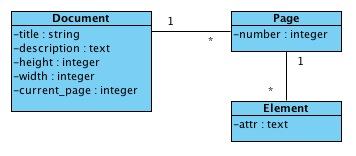
\includegraphics{uml1.png}
\caption{Clases del dominio, 1er ciclo}\label{fig:uml1}
\end{figure}


% subsubsection modelos (end)

\subsubsection{Controladores} % (fold)
\label{ssub:controladores}

En estos momentos se considera suficiente agrupar todas las funcionalidades que traten con los documentos dentro de un solo controlador, \texttt{documents\_controller}. 

% subsubsection controladores (end)

% subsection diseño (end)

\subsection{Implementación} % (fold)
\label{sub:implementacion}

Para inicializar una aplicación en rails, hay que crear dicha aplicación, y configurar la conexión con la base de datos. Desde el principio, se le ha dado el nombre \texttt{drawme}. 

\begin{verbatim}
rails drawme
\end{verbatim}

\subsubsection{Modelos} % (fold)
\label{ssub:modelos}

Este comando generará los archivos que formen el esqueleto de la aplicación. Una vez hecho esto, hay que generar los modelos que se han planeado:

\begin{verbatim}
script/generate model Document
script/generate model Page
script/generate model Element
\end{verbatim}

Estos comandos generarán los archivos dentro de la carpeta \texttt{/app/models}, además de las \emph{migraciones} correspondientes para crear las tablas en la base de datos. Una migración es una acción sobre la base de datos, de cualquier tipo. Dentro de la carpeta \texttt{/db/migrations} se encuentran, ordenadas de forma temporal mediante un timestamp. Gracias a esto se pueden ir realizadno modificaciones sobre la base de datos de forma ordenada, permitiendo así, por ejemplo, que si en un futuro se pretende realizar una modificación, no se tenga que eliminar la base de datos entera y volverla a crear.

A forma de ejemplo, la migración para la tabla del modelo \texttt{Document} será así:

\begin{verbatim}
  class CreateDocuments < ActiveRecord::Migration
    def self.up
      create_table :documents do |t|
        t.string :title
        t.text :description
        t.integer :current_page, :default => 1
        t.integer :height, :default => 600
        t.integer :width, :default => 800
        t.timestamps
      end
    end

    def self.down
      drop_table :documents
    end
  end
\end{verbatim}

Ya en este punto se empieza a notar el concepto de \emph{convention over configuration}, en que se ha creado el modelo \texttt{Document}, y la migración generada llama a la tabla de la base de datos \texttt{documents}. Ésto siempre es así, un modelo es un nombre en singular, y su tabla es el equivalente en plural. Sabiendo esto, no habrá en ningún momento problemas de nomenclatura, y en caso de que sea necesario llamar a una tabla con un nombre distinto al de su modelo, será necesario añadir una línea en su modelo correspondiente (en este caso \texttt{/app/models/document.rb}).

Un documento puede tener múltiples páginas, y es bien sabido que este tipo de relaciones, para ser representadas en una base de datos relacional, hay que añadir una clave externa en la tabla de las páginas. Para hacer esto, en Ruby on Rails se haría lo siguiente:

\begin{verbatim}
  class CreatePages < ActiveRecord::Migration
    def self.up
      create_table :pages do |t|
        t.integer :number, :null => false
        t.references :document
        t.index :document_id
        
        t.timestamps
      end
    end

    def self.down
      drop_table :pages
    end
  end
\end{verbatim}

Esta migración es totalmente autoexplicativa. Por convención, los campos que referencian otra tabla, tienen la nomenclatura \texttt{modelo\_id}, y se aprovecha en este caso para añadir un índice sobre este campo, para que cuando sea necesario consultar las páginas de un documento, no sea necesario recorrer la tabla entera.

La migración para \texttt{Element} es igual a la de \texttt{Page}.

\begin{verbatim}
  class CreateElements < ActiveRecord::Migration
    def self.up
      create_table :elements do |t|
        t.text :attr, :null => false 
        t.references :page
        t.index :page_id

        t.timestamps
      end
    end

    def self.down
      drop_table :elements
    end
  end
\end{verbatim}

Para trasladar estas migraciones a la base de datos es necesario ejecutar la línea siguiente en la línea de comandos:

\begin{verbatim}
  rake db:migrate
\end{verbatim}

Estas migraciones, no obstante, solamente sirven para tratar con la base de datos. Para que la aplicación sepa que un \texttt{Document} tiene múltiples \texttt{Pages}, es necesario dejar constancia en los modelos:

\begin{verbatim}
  class Document < ActiveRecord::Base
    has_many :pages, :dependent => :destroy
    has_many :elements, :through => :pages
  end
\end{verbatim}

\begin{verbatim}
  class Page < ActiveRecord::Base
    has_many :elements, :dependent => :destroy
    belongs_to :document
  end
\end{verbatim}

\begin{verbatim}
  class Element < ActiveRecord::Base
    belongs_to :page
    belongs_to :document, :through => :page
  end
\end{verbatim}


Con estas líneas, será posible en un futuro, ejecutar instrucciones como las siguientes:

\begin{verbatim}
  document.pages << Page.new  # Añadir una página a un documento
  page.elements << Element.create(:attr => "...")  # Añadir un elemento a una página
  document.pages.clear # Borrar todas las páginas de un documento
\end{verbatim}

Cualquier operación que trate las relaciones entre estos elementos será posible de forma tan sencilla, siempre tratando con la base de datos de forma transparente. 

% subsubsection modelos (end)

\subsubsection{Controladores y vistas} % (fold)
\label{ssub:controlador}

De forma similar a los modelos, para generar los archivos necesarios para un controlador:

\begin{verbatim}
  script/generate controller Documents
\end{verbatim}

El archivo generado, utilizando las convenciones, será \texttt{/app/controllers/documents\_controller.rb}. Dentro de este archivo, cada función implementada tendrá una traducción directa en las capa de vistas, por lo tanto el proceso de implementar acciones en controladores suele ir al mismo ritmo que se van implementando las vistas.

Debido a que es el primer ciclo, y que de momento aún no se tiene muy claro cómo acabará estructurándose la web, se optará por tener lo que en Rails se llama un \emph{Scaffold}, con unas pocas modificaciones, para poder editar los documentos. Un Scaffold es una envoltura para un modelo, con las cuatro operaciones básicas que se pueden querer realizar: crear, mostrar, modificar y borrar (\texttt{create}, \texttt{show}, \texttt{update} y \texttt{destroy}). Debido a la naturaleza de la web, es necesario otras acciones, previas a estas cuatro. Por ejemplo, antes de crear un Documento, es necesario mostrar un formulario en el que rellenar los datos necesarios. Dicha acción se llamaría \texttt{new}. Para poder mostrar un elemento en concreto, primero hay que listar los que hay, y dicha acción se llama \texttt{index}. Para poder modificar un elemento primero hay que mostrar como está en este instante, además de proporcionar un formulario con el que poder especificar los cambios. Ésta acción se llamaría \texttt{edit}. Para eliminar un elemento solo es necesario saber qué elemento eliminar, por lo tanto es posible ejecutar tanto desde \texttt{show} como desde \texttt{index}.

Éstas cuatro acciones forman el llamado \texttt{CRUD} (Create, Retrieve, Update y Delete), y equivalen a las cuatro comentadas, que junto con las otras tres, forman las siete acciones básicas de un controlador de Scaffold.

Puesto que estas acciones son tan comunes, Rails proporciona una forma de generar un Scaffold sencillo de forma totalmente automática, para utilizar como punto de partida.

\begin{verbatim}
  script/generate scaffold Document
\end{verbatim}

Gracias a las convenciones de Rails, este Scaffold buscará el modelo \texttt{Document} y creará el controlador \texttt{documents\_controller} con el código adecuado, y las vistas correspondientes.

Este scaffolding, sin embargo, no tiene en cuenta las relaciones entre modelos, ni ningún comportamiento personalizado que se quiera tener. Así, los cambios necesarios para adecuar este scaffold al gusto de la aplicación serían los siguientes:

\begin{itemize}
  \item En el momento de crear un documento, añadirle un número fijo de páginas vacías, con sus números de páginas correspondientes.
  \item El atributo \texttt{current\_page} no debe ser editable, de momento, puesto que se manejará mediante la interfaz javascript.
\end{itemize}

Con estos sencillos pasos se puede considerar la primera funcionalidad objetivo cumplida. La segunda funcionalidad es permitir tratar con la interfaz, mediante la comunicación con ajax y transportando elementos en formato JSON. Las funciones necesarias para ello se pueden resumir en las siguientes:

\begin{description}
  \item[\texttt{add\_element}] recibiendo para qué página (y por consiguiente, qué documento), y el objeto en JSON, y retornando el identificador del mismo una vez guardado.
  \item[\texttt{remove\_element}] recibiendo el identificador del elemento.
  \item[\texttt{list\_elements}] recibiendo la página (y por consiguiente, el documento), devolviendo el listado de elementos en formato JSON.
  \item[\texttt{change\_page}] recibiendo la página a la que se quiere cambiar.
\end{description}

Cabe destacar de la implementación de estas funciones, la facilidad que da Rails para tratar con peticiones en Ajax. En el caso de la función \texttt{list\_elements}, por ejemplo, lo lógico sería realizar una búsqueda en la base de datos, teniendo luego un vector de elementos, que luego se deberían traducir a JSON, y mostrarse en la vista.

\begin{verbatim}
  def list_elements
    elements = Page.find(params[:page_id]).elements
    render :json => elements
  end
\end{verbatim}

Debido a que JSON se ha convertido en un formato standard en este tipo de acciones, Rails usa las librerías de Ruby para la conversión de objetos a sus equivalentes en JSON, y mediante una sola línea es posible devolver un objeto exactamente equivalente al que se tiene en ese momento en Ruby, pero que javascript podrá entender.

Con esto, se tienen las dos funcionalidades originales, y ya sería posible empezar a dibujar en la interfície en Javascript, con múltiples usuarios al mismo tiempo, todo con presistencia en una base de datos, y todo con una simplicidad extrema.

% subsubsection controlador (end)

% subsection implementacion (end)
% section primer_ciclo (end)
\newpage
%!TEX root = /Users/simo/Documents/PFC/memoria/memoria.tex
\section{Segundo Ciclo} % (fold)
\label{sec:secundo_ciclo}

Se considera interesante que la siguiente evolución de la aplicación sea la introducción del concepto de Usuario.

\subsection{Análisis de requisitos} % (fold)
\label{sub:análisis_de_requisitos}

\begin{itemize}
  \item Poder registrarse en la web de la forma más simple posible.
  \item Tener un panel sencillo desde el que manejar sus documentos
  \item Seguridad básica para que no se pueda acceder a elementos que no se debería tener acceso.
\end{itemize}

% subsection análisis_de_requisitos (end)

\subsection{Diseño} % (fold)
\label{sub:diseño}

En cuanto al diagrama de clases del dominio, en este caso aparece un nuevo modelo usuario \texttt{User}, el cual tiene varios \texttt{Document}'s, y tiene los atributos básicos de nombre de usuario (\texttt{login}), \texttt{email} y \texttt{password}.

\begin{figure}[h!]
\centering
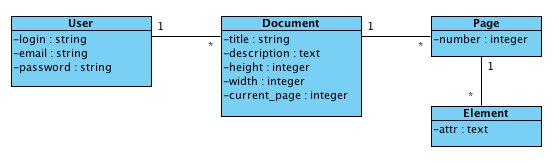
\includegraphics[width=15cm]{uml2.png}
\caption{Clases del dominio, 2º ciclo}\label{fig:uml2}
\end{figure}

Para manejar todo el proceso de registro, y cualquiera del resto de acciones necesarias, si llegara el caso de recuperar contraseña, dar de baja, o editar los datos de usuario, se cree necesario crear otro controlador diferente, al que se llamará \texttt{users\_controller}. También, al tener en este caso una parte privada y una parte pública de la web, es necesario tener una serie de acciones que no tienen que ver ni con manejar documentos ni con registrarse. Por ello, y para cualquier otra acción sencilla que se quiera añadir en un futuro referente a lo que sería la web en si (página de contacto, ayuda, información del autor, etc), se ha decidido crear un controlador extra llamado \texttt{website\_controller}.

% subsection diseño (end)

\subsection{Implementación} % (fold)
\label{sub:implementación}

\subsubsection{Registro de usuarios} % (fold)
\label{ssub:registro_de_usuarios}

El proceso de manejo de usuarios es un tema muy delicado en cuanto a seguridad se refiere. Existen sobradas razones para blindar totalmente este proceso, que la contraseña esté guardada de forma encriptada, y que los datos que introduce el usuario estén seguros. Y puesto que la funcionalidad de poder registrarse en una web es algo tan común en el mundo de las webs, existe alguien que se ha encargado de facilitar todo este proceso en forma de plugin para Rails.

Los plugins pueden servir para multitud de propósitos, y suelen solucionar necesidades comunes de las webs que Rails no incluye para no sobrecargar el Framework. En este caso el plugin se llama \texttt{restful\_authentication} \footnote{\url{http://github.com/technoweenie/restful-authentication}}. Este plugin se encarga de las tareas de registro de usuarios creando un modelo llamado User, tal y como se había planeado, y un controlador con las funciones de registro (\texttt{signup}), login y logout. Además, aporta una serie de funciones de ayuda (\texttt{helpers} en Rails), que permiten tratar en todo momento con el usuario, y por ejemplo, saber si la persona que está realizando una petición de una página está logueado o no. 

Este plugin utiliza la técnica de salted passwords \footnote{\url{http://en.wikipedia.org/wiki/Salt\_(cryptography)}} para almacenar las contraseñas en la base de datos. Ésta técnica genera una cadena aleatoria (salt) de 40 caracteres mediante \texttt{SHA1}, que se utiliza para generar el llamado salted password, también de 40 caracteres mediante \texttt{SHA1}. Se considera el standard de facto en cuanto a registro y guardado de contraseñas se refiere, y es una técnica utilizada en numerosos protocolos criptográficos, como por ejemplo SSL. Esta encriptación dificulta los ataques a contraseñas mediante diccionario de forma exponencial, puesto que por cada palabra \emph{común} de los diccionarios usados, es necesario tener las $2^{160}$ posibles combinaciones introducidas por el salt de 160 bits. Incluso si la base de datos se comprometiera, y un atacante tuviera acceso a alguno de los campos, tanto el salt, como el password encriptado, aún debería romper la clave mediante el método tradicional, puesto que ya sabría cual es el salt, pero seguiría teniendo que encontrar cual es la clave que, añadida al salt, y encriptándola mediante SHA1, genera el password encriptado.

Este plugin requiere de el campo extra salt, que no se había planteado en un principio en la etapa de diseño.

% subsubsection registro_de_usuarios (end)

\subsubsection{Panel de control} % (fold)
\label{ssub:panel_de_control}

Mediante el plugin de usuarios es cuestión de controlar si se está logueado o no para mostrar la pantalla inicial de la web, del controlador \texttt{website\_controller}, o la pantalla con el \emph{panel de control} del usuario, también dentro del mismo controlador. El siguiente paso es evolucionar el Scaffold de documentos para controlar que en todo momento, solo el propietario de los documentos pueda realizar las acciones solicitadas.

Así, por ejemplo, las funciones del \texttt{documents\_controller} evolucionan de unas líneas como las siguientes:

\begin{Verbatim}[commandchars=@\[\]]
  @PYaz[def] @PYaL[update]
    @PYaS[@PYZat[]doc] @PYbf[=] @PYar[Document]@PYbf[.]find(params@PYbf[@PYZlb[]]@PYau[:id]@PYbf[@PYZrb[]])
    @PYaS[@PYZat[]doc]@PYbf[.]update_attributes params@PYbf[@PYZlb[]]@PYau[:document]@PYbf[@PYZrb[]]
    redirect_to @PYau[:action] @PYbf[=]@PYbf[>] @PYaX["]@PYaX[edit]@PYaX["], @PYau[:id] @PYbf[=]@PYbf[>] @PYaS[@PYZat[]doc]@PYbf[.]id
  @PYaz[end]
\end{Verbatim}


%\begin{verbatim}
%  def update
%    @doc = Document.find(params[:id])
%    @doc.update_attributes params[:document]
%    redirect_to :action => "edit", :id => @doc.id
%  end
%\end{verbatim}

A algo como lo siguiente:

\begin{Verbatim}[commandchars=@\[\]]
  @PYaz[def] @PYaL[update]
    @PYaS[@PYZat[]doc] @PYbf[=] @PYar[Document]@PYbf[.]find(params@PYbf[@PYZlb[]]@PYau[:id]@PYbf[@PYZrb[]])
    redirect_to @PYau[:action] @PYbf[=]@PYbf[>] @PYau[:index] @PYaz[unless] @PYaS[@PYZat[]doc]@PYbf[.]user @PYbf[==] current_user
    @PYaS[@PYZat[]doc]@PYbf[.]update_attributes params@PYbf[@PYZlb[]]@PYau[:document]@PYbf[@PYZrb[]]
    redirect_to @PYau[:action] @PYbf[=]@PYbf[>] @PYaX["]@PYaX[edit]@PYaX["], @PYau[:id] @PYbf[=]@PYbf[>] @PYaS[@PYZat[]doc]@PYbf[.]id
  @PYaz[end]
\end{Verbatim}

%\begin{verbatim}
%  def update
%    @doc = Document.find(params[:id])
%    redirect_to :action => :index unless @doc.user == current_user
%    @doc.update_attributes params[:document]
%    redirect_to :action => "edit", :id => @doc.id
%  end
%\end{verbatim}

Dichos cambios son mínimos, por la simplicidad en que todos ellos están implementados. La parte de comunicación con Javascript, de momento, se dejará abierta hasta que se decida qué política se aplicará para permitir o no a los usuarios ver o editar sus contenidos.

% subsubsection panel_de_control (end)

% subsection implementación (end)

% section secundo_ciclo (end)
\newpage
%!TEX root = /Users/simo/Documents/PFC/Chapter3/chapter3.tex
\section{Tercer Ciclo} % (fold)
\label{sec:tercer_ciclo}

En estos momentos un usuario puede crear y editar sus documentos, pero aún no existe ningún tipo de seguridad a la hora de trabajar desde la pizarra. La idea original para esta aplicación, es que los usuarios podrían acceder a documentos dependiendo de los permisos que se le hubiera dado, tanto por la parte del grupo como independientemente. Para este ciclo, el objetivo será la introducción del concepto Grupo, de forma que se puedan agrupar usuarios de forma sencilla y rápida, y que se puedan asignar en un futuro, permisos de forma rápida a estos grupos de gente.

\subsection{Análisis de requisitos} % (fold)
\label{sub:análisis_de_requisitos}

\begin{itemize}
  \item Poder crear, editar y borrar grupos.
  \item Un grupo deberá tener un dueño, que será el creador, que siempre tendrá los máximos permisos, y que podrá invitar, echar y promocionar a otros usuarios. Una vez invitado, un miembro puede ser promocionado a administrador, de forma que pueda a su vez, invitar, promocionar y echar a gente. Un administrador no puede eliminar el grupo o echar / degradar a otros administradores, privilegios reservados al dueño del grupo.
  \item Los usuarios invitados pueden aceptar o rechazar las invitaciones, además de salir del grupo voluntariamente, después de ser invitado. Para evitar una avalancha de invitaciones, solo un usuario puede invitar a un usuario a un grupo.
\end{itemize}

% subsection análisis_de_requisitos (end)

\subsection{Diseño} % (fold)
\label{sub:diseño}

\begin{figure}[h!]
\centering
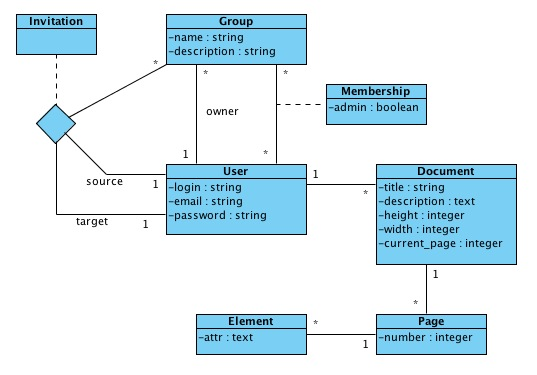
\includegraphics[width=14cm]{uml3.png}
\caption{Clases del dominio, 3er ciclo}\label{fig:uml3}
\end{figure}

En este paso se hace todo el sistema de clases un tanto más complejo. Un grupo tiene una relación doble con la clase \texttt{User}, teniendo un dueño, y múltiples usuarios. Además, puesto que los miembros pueden ser administradores, existen dos posibilidades. Una sería tener una triple relación, de dueño, administradores y usuarios normales; la otra sería tener una clase asociativa \texttt{Membership}, que contenga la información de si este miembro tiene permisos de administrador o no. La segunda opción se cree más eficiente, puesto que siempre será más fácil modificar un atributo de la tabla \texttt{Membership} que destruir una relación y crear otra nueva, además de simplificar el proceso de encontrar todos los miembros de un grupo, sean administradores o no.

En cuanto al proceso de realizar invitaciones, es necesario almacenar de alguna forma temporal dichas invitaciones, y la solución natural es una asociación ternaria entre un grupo y dos usuarios, el que invita (source) y el invitado (target).

Ruby on Rails aún no soporta relaciones asociativas, debiéndose por tanto normalizar el diagrama antes de poder traducirse a la estructura de modelos.

\begin{figure}[h!]
\centering
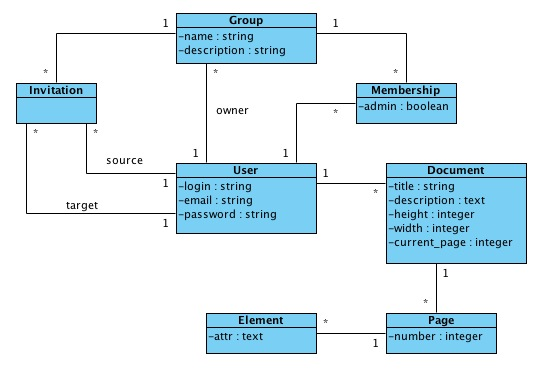
\includegraphics[width=14cm]{uml3n.png}
\caption{Clases del dominio, 3er ciclo, diagrama normalizado}\label{fig:uml3n}
\end{figure}

En cuanto a modelos, se cree necesario crear un nuevo controlador para todas las acciones referentes a los grupos

% subsection diseño (end)

\subsection{Implementación} % (fold)
\label{sub:implementación}

A pesar de la nueva complejidad de las clases introducidas (tres nuevas clases, con un total de seis nuevas relaciones), el proceso de traducción de este diagrama a clases es puramente burocrático. El peso de controlar las restricciones dejadas atrás por la normalización recae sobre los controladores, que a la hora de invitar a gente se deberá comprobar que no sea miembro y que no haya sido invitado ya, todo sostenido sobre un Scaffold para los grupos, de la misma forma que se ha hecho con los documentos, pero con un pequeño extra de complejidad.

La forma de organizar todas estas nuevas funcionalidades es mostrando una lista de grupos (acción \texttt{index} del Scaffold) dentro del panel de control, de la misma forma que los documentos, y que al ir a editar un grupo se muestre un formulario si eres administrador, o una vista simple si no se es. De la misma forma, el pequeño formulario para invitar a gente solo aparecerá si el usuario es administrador. En cuanto a los usuarios invitados, cuando se entre en el panel, en caso de que haya sido invitado a algún grupo, se le mostrará un mensaje con el nombre de usuario de la persona que ha invitado y el nombre del grupo, con opción de aceptar o rechazar.

% subsection implementación (end)

% section tercer_ciclo (end)
\newpage
%!TEX root = /Users/simo/Documents/PFC/Chapter3/chapter3.tex
\section{Cuarto Ciclo} % (fold)
\label{sec:cuarto_ciclo}

Una vez se tiene el concepto de Grupo introducido en el sistema, está todo preparado para poder generar todo el sistema de permisos para la interfaz Javascript.

\subsection{Análisis de requisitos} % (fold)
\label{sub:análisis_de_requisitos}

\begin{itemize}
  \item Individualmente para cada documento, se debe poder definir una lista de usuarios y grupos que pueden \emph{participar} en este documento, definiendo para cada uno de estos si participan en calidad de espectador o de ponente. Un ponente puede \emph{dibujar} en la pizarra, los espectadores solo reciben los cambios hechos en las pizarra.
  \item Además, se debe poder hacer una pizarra pública, de forma que cualquier usuario pueda participar en forma de espectador.
\end{itemize}

% subsection análisis_de_requisitos (end)

\subsection{Diseño} % (fold)
\label{sub:diseño}

El concepto de permisos es semejante al concepto de invitaciones, siendo la única diferencia que no es algo que se pueda rechazar. El creador del documento puede añadir o quitar conexiones entre un documento y un usuario o grupo, que además deberá constatar si es en forma de ponente o de observador, necesitando pues, una clase asociativa.

\begin{figure}[h!]
\centering
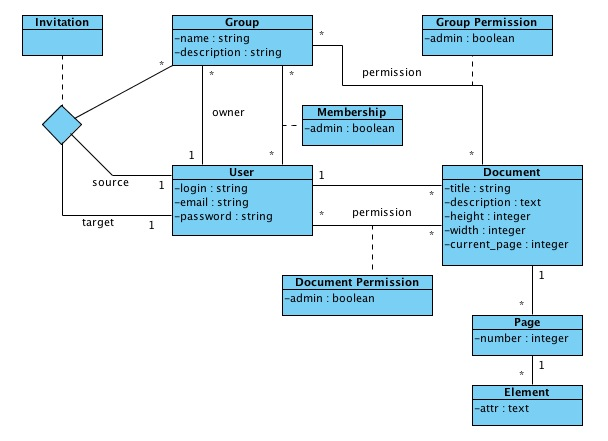
\includegraphics[width=14cm]{uml4.png}
\caption{Clases del dominio, 4º ciclo}\label{fig:uml4}
\end{figure}

Y por lo tanto, normalizado:

\begin{figure}[h!]
\centering
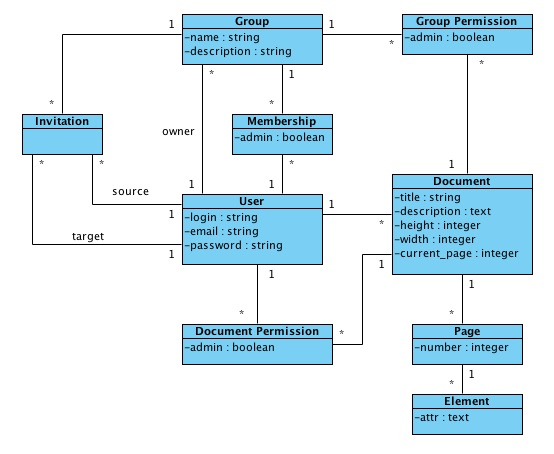
\includegraphics[width=14cm]{uml4n.png}
\caption{Clases del dominio, 4º ciclo, diagrama normalizado}\label{fig:uml4n}
\end{figure}

% subsection diseño (end)

\subsection{Implementación} % (fold)
\label{sub:implementación}

De nuevo, traducir estas dos nuevas clases a modelos de Rails no es más que un proceso repetitivo y tremendamente sencillo. El proceso de integrar estas nuevas funcionalidades en el sistema, es más un problema de encontrar una interfaz adecuada para todas estas operaciones, que de implementación de los controladores.

Finalmente el diagrama de clases se ha convertido en algo más grande, e incluso con las facilidades que ofrece Rails para manejar todas estas relaciones, es importante mantener todo bien organizado. Se considera una buena práctica tener la mayor parte del código implementada en los modelos. Ésto es así puesto que una función implementada en un modelo siemre es reutilizable, y poniéndose un límite de unas 10 líneas de código en cada función del controlador, hace que se tenga en todo momento unas acciones bien claras y definidas, y por lo tanto, de muy fácil modificación en futuras iteraciones.

Así pues, lo más fácil es implementar funciones como las siguientes:

\begin{verbatim}
  document.can_be_seen_by?(user)
  document.can_be_edited_by?(user)
  document.can_be_deleted_by?(user)
  user.all_accessible_documents
  user.invite(user,group)
  group.is_member?(user)
  group.is_admin?(user)
  group.is_owner?(user)
  group.add_user(user)
  group.promote(user)
  group.unpromote(user)
\end{verbatim}

Todas son completamente autoexplicativas gracias a sus nombres, y contribuyen a que los controladores simplifiquen la mayoría de su código dejando solamente las líneas esenciales para que cualquier programador pueda saber de un vistazo qué hace este controlador.

Teniendo estas funciones implementadas, modificar las cuatro acciones de comunicación con el motor para tenerlas en cuenta, no necesita más que una línea extra.

% subsection implementación (end)

% section cuarto_ciclo (end)
\newpage
%!TEX root = /Users/simo/Documents/PFC/memoria/memoria.tex
\section{Quinto Ciclo} % (fold)
\label{sec:quinto_ciclo}

En este ciclo se pretende tratar un tema que se ha ignorado desde el principio, que es la subida de archivos (pdf's o imágenes) para hacer de fondo en las páginas de los documentos. Debido a la naturaleza compleja de la tarea se ha preferido dejar para las últimas etapas del desarrollo, cuando hubiera una comprensión mayor del funcionamiento de Ruby on Rails.

\subsection{Análisis de requisitos} % (fold)
\label{sub:análisis_de_requisitos}

\begin{itemize}
  \item Poder crear páginas en blanco.
  \item Poder subir imágenes una a una creando páginas para el documento con ellas.
  \item Poder subir archivos comprimidos con imágenes dentro, que creen una página por cada imagen que se encuentre en el archivo. Las páginas se deberían ordenarán alfabéticamente según el nombre del archivo de la imagen. Como opción básica, se debe poder subir archivos zip, pero idealmente se debería poder subir otros formatos comunes, como rar o gz.
  \item Poder subir PDF's, que automáticamente convertirían cada página a una imagen, asignándola a una página nueva.
\end{itemize}

% subsection análisis_de_requisitos (end)

\subsection{Diseño} % (fold)
\label{sub:diseño}

\begin{figure}[h!]
\centering
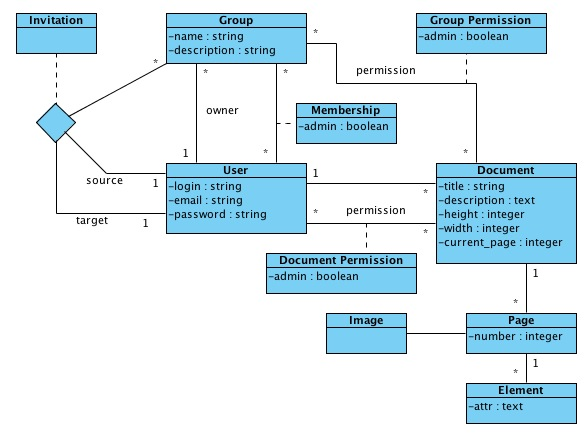
\includegraphics[width=14cm]{uml5.png}
\caption{Clases del dominio, 5º ciclo}\label{fig:uml5}
\end{figure}

Debido a lecturas en ciclos anteriores se conoce que el proceso de subir imágenes es otro aspecto muy común de las páginas web, y por lo tanto existe un Plugin excelente que da todas las herramientas necesarias para subir, generar thumbnails y almacenar imágenes en distintos soportes. Estos plugins generalmente requieren de un modelo extra que representará las imágenes, y que, como cualquier otro modelo dentro de Rails, se puede relacionar con el resto. Por tanto, aprovechando este conocimiento, se puede planear ya este modelo, y asignarlo, lógicamente, al modelo \texttt{Page}.

Este modelo solo tiene los atributos creados por el plugin, por lo cual se obvian en beneficio de una mayor claridad del diagrama.

% subsection diseño (end)

\subsection{Implementación} % (fold)
\label{sub:implementación}

La forma en que se plantearán estas funcionalidades, serán mostrando una columna lateral en la edición de un documento, separada del formulario de edición del documento y de administración de permisos, mediante el cual se mostrarían miniaturas de las páginas, y se podrían ir añadiendo páginas mediante las opciones disponibles. 

\subsubsection{Páginas en blanco} % (fold)
\label{ssub:paginas_en_blanco}

Esta es la opción más sencilla, y no necesita más que una acción que cree una página de la misma forma que se creaban anteriormente, cuando se generaba una cantidad de páginas fija. De la misma forma, es posible añadir una opción para generar un número de páginas, establecido por el usuario rellenando un campo de texto.

% subsubsection paginas_en_blanco (end)

\subsubsection{Subir imágenes una a una} % (fold)
\label{ssub:subir_imagenes_una_a_una}

Esta opción es el ejemplo clásico de uso de un plugin para subir archivos. El plugin utilizado en este caso es \texttt{attachment-fu} \footnote{\url{http://github.com/technoweenie/attachment\_fu}} , el cual, añadiendo unas líneas como las siguientes, hace que se relacione directamente con los archivos subidos mediante la interfaz web.

\begin{Verbatim}[commandchars=@\[\]]
@PYaz[class] @PYaO[Image] @PYbf[<] @PYar[ActiveRecord]@PYbf[::]@PYar[Base]
  belongs_to @PYau[:page]
  
  has_attachment  @PYau[:content_type] @PYbf[=]@PYbf[>] @PYau[:image],
                  @PYau[:processor] @PYbf[=]@PYbf[>] @PYbe['MiniMagick'],
                  @PYau[:thumbnails] @PYbf[=]@PYbf[>] {@PYau[:small] @PYbf[=]@PYbf[>] @PYbe['85x>'],
                                  @PYau[:medium] @PYbf[=]@PYbf[>] @PYbe['360x360>'],
                                  @PYau[:big] @PYbf[=]@PYbf[>] @PYbe['800x800>']},
                  @PYau[:storage] @PYbf[=]@PYbf[>] @PYau[:file_system],
                  @PYau[:path_prefix] @PYbf[=]@PYbf[>] @PYaX["]@PYaX[/document_images/]@PYaX["]
@PYaz[end]
\end{Verbatim}

%\begin{verbatim}
%class Image < ActiveRecord::Base
%  belongs_to :page
%  
%  has_attachment  :content_type => :image,
%                  :processor => 'MiniMagick',
%                  :thumbnails => {:small => '85x>',
%                                  :medium => '360x360>',
%                                  :big => '800x800>'},
%                  :storage => :file_system,
%                  :path_prefix => "/document_images/"
%end
%\end{verbatim}

Introduciendo esto en \texttt{/app/models/image.rb}, y al crear un objeto de tipo Image, pasándole como parámetro el input en el que se el usuario añade el archivo, hará las siguientes acciones:

\begin{itemize}
  \item Comprobará que es una imagen, porque se le ha pasado el parámetro \texttt{:content\_type => :image}. En caso de no ser un archivo de tipo imagen válido, fallará el momento de crear el objeto, es decir, al realizar un \texttt{save} o un \texttt{create} sobre \texttt{Image}.
  \item Generará tres thumbnails, con los tamaños especificados usando el formato clásico de \texttt{ImageMagick} \footnote{\url{http://imagemagick.org/script/command-line-options.php\#resize}}, mediante \texttt{MiniMagick} \footnote{\url{http://rubyforge.org/projects/mini-magick/}}.
  \item Guardará las imágenes en la carpeta \texttt{/document\_images}. Puesto que se le ha especificado claramente que está en la raíz de la aplicación, las guardará ahí, y no en \texttt{public}, que es lo normal. \texttt{public} es la carpeta que está abierta al público, y si se guardara en \texttt{/public/document\_images} en vez de en \texttt{/document\_images}, cualquier persona podría acceder a las imágenes mediante la dirección pública como \texttt{http://dominio.com/document\_images/..}
  
  De esta forma las imágenes están fuera del alcance, y se deberán servir mediante un método que lea este archivo y lo transmita, que al ser programado especialmente, puede controlar que el usuario que está reclamando una imagen tenga permisos para ver el documento, y no esté intentando ver documentos del resto.
\end{itemize}

Con la siguiente instrucción:

%\begin{verbatim}
%  send_file :file => image.public_filename(params[:thumb])
%\end{verbatim}

\begin{Verbatim}[commandchars=@\[\]]
  send_file @PYau[:file] @PYbf[=]@PYbf[>] image@PYbf[.]public_filename(params@PYbf[@PYZlb[]]@PYau[:thumb]@PYbf[@PYZrb[]])
\end{Verbatim}


es posible renderizar dicha imagen, de la misma forma que si accediera desde la dirección pública, pero estando dicha imagen fuera del alcance de todo el mundo, y pudiendo realizar las comprobaciones pertinentes.

% subsubsection subir_imagenes_una_a_una (end)

\subsubsection{Subiendo imágenes en un archivo comprimido} % (fold)
\label{ssub:subiendo_imágenes_en_un_archivo_comprimido}

Esta segunda opción añade una complicación básica, en que ninguno de los plugins existentes permiten hacer nada parecido a lo necesario aquí, por lo que debe hacerse todo a mano. La forma en que funcionan las subidas mediante web, en cualquier sistema, es que el servidor genera un archivo temporal conteniendo el archivo en si, y que Ruby on Rails permite acceder de forma normal, igual que se accede a cualquiera de los parámetros rellenados en un formulario, pero en vez de ser un \texttt{String}, es un \texttt{Tempfile} \footnote{\url{http://corelib.rubyonrails.org/classes/Tempfile.html}}. 

Puesto que es un archivo que se deberá descomprimir, y después realizar las acciones necesarias para generar páginas con las imágenes descomprimidas, es necesario algún tipo de organización de directorios para poder trabajar de forma temporal, y sin que pueda haber interferencias entre varios procesos descomprimiendo al mismo tiempo. La carpeta \texttt{/document\_temp} contendrá una serie de carpetas que se irán creando cuyo nombre será el timestamp del momento de la subida, concatenado con el identificador del documento para el cual se están subiendo imágenes. De esta forma, se puede en un futuro tener un control de carpetas que quizá hayan quedado descontroladas por algún proceso interrumpido de forma inesperada, siempre controlado que por ejemplo, dichas carpetas temporales hayan sido creadas hace más de una hora.

Dicha previsión se cree conveniente para poder blindar el proceso, y que ningún posible error en el código, o subidas de archivos maliciosos puedan ocupar espacio indeseado.

Mediante Ruby, igual que con cualquier otro lenguaje, es posible realizar todo tipo de operaciones de movimiento de archivos y creación de carpetas, por lo que crear dicha carpeta y eliminarla al final no es problema. El siguiente reto es conseguir descomprimir un archivo, en principio, desconocido, y por supuesto, contra más flexibilidad mejor. Existe un descompresor llamado \texttt{e}, de Martin Ankerl \footnote{\url{http://martin.ankerl.com/2006/08/11/program-e-extract-any-archive/}}, que al estar escrito en Ruby, es muy fácilmente adaptable a las necesidades de este proyecto. El código utilizado por este descompresor soporta hasta un límite de 32 formatos distintos, siempre y cuando esté el descompresor necesario instalado en el sistema.

Una vez descomprimidas las imágenes, existe el problema de la organización interna del fichero. ¿Qué pasa si existen varias carpetas? En este punto se corre el riesgo de complicar extremadamente la cosa, puesto que no siempre se puede saber cuál es la intención del usuario a la hora de subir las imágenes comprimidas en varias carpetas. En este caso, se ha tomado la política de extraer todas las imágenes, independientemente de la carpeta en que estén, y añadirlas de forma ordenada alfabéticamente.

Para hacer esto, de nuevo, aparentemente complejo, no hay más que usar uno de los módulos de la librería básica de Ruby, \texttt{Find} \footnote{\url{http://corelib.rubyonrails.org/classes/Find.html}}, el cual permite recorrer recursivamente una estructura de directorios, a partir de la cual generar un vector de archivos, referenciables posteriormente. Mediante este vector, y la función \texttt{File.basename}, es posible ordenar los archivos, guardados en el vector \texttt{files}, con la siguiente línea:

\begin{Verbatim}[commandchars=@\[\]]
files@PYbf[.]sort! {@PYbf[|]a,b@PYbf[|] @PYar[File]@PYbf[.]basename(a) @PYbf[<]@PYbf[=]@PYbf[>] @PYar[File]@PYbf[.]basename(b)}
\end{Verbatim}

%\begin{verbatim}
%  files.sort! {|a,b| File.basename(a) <=> File.basename(b)}
%\end{verbatim}

Ruby, de nuevo, ya tiene un algoritmo de ordenación implementado, al cual se le puede explicar por qué parámetro ordenar un vector, en este caso, por los nombres de archivo.

Teniendo, pues, un vector con referencias a las imágenes, ya comprimidas y ordenadas alfabéticamente solo queda generar las páginas con sus elementos \texttt{Image} generados. Mediante otra línea de texto explicada en la documentación del plugin \texttt{attachment-fu}, es fácilmente generable objetos de este tipo a partir de archivos ya existentes en el servidor.

% subsubsection subiendo_imágenes_en_un_archivo_comprimido (end)

\subsubsection{Subiendo archivos PDF} % (fold)
\label{ssub:subiendo_archivos_pdf}

Éste, a pesar de lo que pueda parecer, es un problema muy semejante al proceso anterior. El proceso de convertir de un archivo PDF a imágenes es posible gracias a la herramienta \texttt{ImageMagick}, un standard de facto en cualquier servidor web para el proceso de imágenes, que se ha usado tradicionalmente para la generación de thumbnails, redimensionado de imágenes, ademas de otras tareas un tanto más avanzadas como la adición de marcas de agua a imágenes. Entre sus posibilidades, existe la posibilidad de convertir entre cualquiera de los formatos soportados, encontrándose PDF entre ellos. Convertir de un PDF a una serie de imágenes es posible mediante el comando:

\begin{verbatim}
  $ convert file.pdf image.jpg
\end{verbatim}

Generando una imagen por página con los nombres \texttt{image0.jpg}, \texttt{image1.jpg}, etc. Teniendo, pues, estas imágenes descomprimidas en un directorio, no hay más que seguir el mismo proceso que con las imágenes descomprimidas para crear las páginas necesarias.

\begin{figure}[h!]
\centering
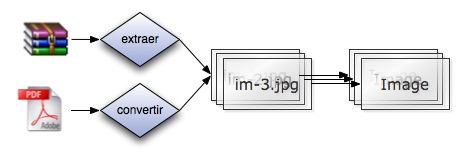
\includegraphics[totalheight=5cm]{converter.jpg}
\caption{Diagrama de la generación de Images a partir de PDF's o archivos comprimidos}\label{fig:converter}
\end{figure}


% subsubsection subiendo_archivos_pdf (end)

\subsubsection{Otras posibilidades} % (fold)
\label{ssub:otras_posibilidades}

Una de las posibilidades que se barajó el etapas preliminares del proyecto, fue la posibilidad de subir presentaciones PowerPoint directamente, puesto que es uno de los formatos más usados para presentaciones, y al fin y al cabo el objetivo básico de esta aplicación es facilitar dichas presentaciones cuando deben realizarse a distancia.

Esta tarea, sin embargo, es prácticamente imposible presuponiendo que la aplicación funcionará sobre una plataforma Unix, lo más normal en cualquier servidor web. En caso de estar funcionando en una plataforma Windows, sería posible mediante los componentes OLE32. En cualquier otro caso, este problema no se ha podido resolver.

% subsubsection otras_posibilidades (end)

% subsection implementación (end)

% section cuarto_ciclo (end)
\newpage
%!TEX root = /Users/simo/Documents/PFC/Chapter3/chapter3.tex
\section{Sexto Ciclo} % (fold)
\label{sec:sexto_ciclo}

La siguiente iteración intentará solucionar un problema aparecido en el ciclo anterior, y requiere de un enfoque distinto para el proceso de generación de páginas en masa a partir de PDF's o archivos comprimidos. Pero previa comprensión de las razones por las que puede haber un problema en este proceso, es necesario entender como funciona una web Ruby on Rails en un entorno \emph{real}.

La forma tradicional de mantener un servidor web sirviendo una aplicación desarrollada en Ruby on Rails, es teniendo una o varias instancias de dicha aplicación sirviendo páginas. Cada instancia de dicha aplicación puede servir solamente una página a la vez, pero puesto que están cargadas todas las librerías, y además se utilizan múltiples técnicas de cacheo, y que por tanto no es necesario recargar código después de cada consulta, dichas páginas se sirven de forma extremadamente rápida.

Esto, sin embargo, quiere decir que mientras una aplicación está ocupada sirviendo una petición, no puede atender a otra. Generalmente, páginas normales de la aplicación tienen un tiempo de generación mínimo, pero ante tareas como las que atañen a este ciclo (conversión de PDF's y descompresión de archivos), significan mantener una de dichas instancias ocupadas durante segundos enteros. Así, por tanto, en cuanto hubiera una cantidad de personas subiendo archivos igual a la cantidad de instancias del servidor, nadie podría navegar, pues todas las instancias estarían ocupadas. No solo eso, sino que tener varios procesos realizando operaciones de actividad intensiva de CPU, y que además suelen necesitar de memoria extra, no es una situación deseable.

Éste es un problema similar al que afrontan servicios similares, como podrían ser, por ejemplo, cualquiera de los servicio de subida de vídeos como Youtube o Vimeo, y la solución para estos problemas, es la de tener un proceso a parte dedicado solamente a realizar dichas tareas. Este proceso, al ser solamente uno, evita situaciones en que el sistema pueda estar saturado tanto por no quedar instancias disponibles a los usuarios para seguir visitando la web, como por tener múltiples procesos intensivos de CPU realizándose al mismo tiempo.

\subsection{Análisis de requisitos} % (fold)
\label{sub:análisis_de_requisitos}

\begin{itemize}
  \item Implementar un mecanismo de forma que pueda existir un proceso a parte dedicado a realizar tareas costosas.
  \item Que el código actual utilice dicho sistema.
\end{itemize}

% subsection análisis_de_requisitos (end)

\subsection{Diseño} % (fold)
\label{sub:diseño}

La dinámica de funcionamiento para esta nueva funcionalidad, será la de ir creando tareas que el proceso aparté irá procesando. Es necesario pues, almacenar dichas tareas en la base de datos, con los datos necesarios para poder ser recuperadas y procesadas a posteriori. Este nuevo modelo, al que se llamará \texttt{Task}, aparece en el diagrama de clases que se encuentra en el diagrama \ref{fig:uml6}:

\begin{figure}[h!]
\centering
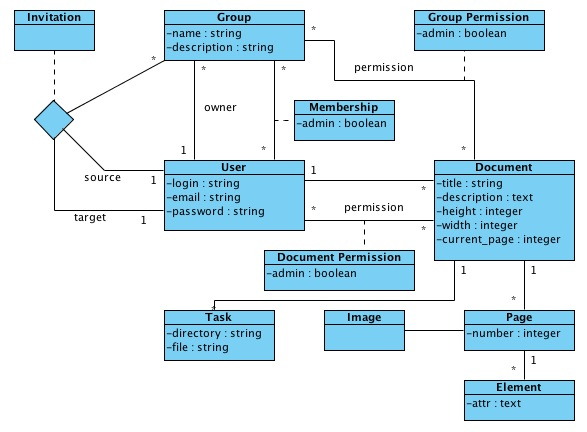
\includegraphics[width=14cm]{uml6.png}
\caption{Clases del dominio, 6º ciclo}\label{fig:uml6}
\end{figure}

% subsection diseño (end)

\subsection{Implementación} % (fold)
\label{sub:implementación}

Este problema, como ya se ha comentado, es muy común en este tipo de servicios, con lo que existe un plugin adecuado, mucho más completo que si esta parte del código se hubiera tenido que programar desde cero. Dicho plugin es \texttt{delayed\_jobs} \footnote{\url{http://github.com/tobi/delayed\_job}}, fruto del trabajo de la web Shopify \footnote{\url{http://www.shopify.com/}}, un servicio de hosting de e-commerce, y que ha publicado su sistema de ejecución de tareas de forma pública en modo de plugin.

Este plugin generaliza mucho más de lo que se había pensado inicialmente, y es capaz de almacenar cualquier tipo de modelo, serializándolo para posterior recuperación, ejecutando siempre la función \texttt{perform}, de forma que con un solo proceso es posible realizar cualquier tipo de tarea que se quiera \emph{separar} del flujo normal de trabajo. En este caso no es necesario, pero es perfectamente adecuado para posibles necesidades en el futuro.

La forma en que funciona es teniendo una tabla propia de tareas, llamadas \texttt{Jobs}, de forma que, en realidad, harían falta dos nuevos modelos para poder desempeñar estos trabajos, pero puesto que el plugin se encarga de almacenar el objeto que debe procesar serializándolo, es posible implementar un modelo que no tenga porqué estar reflejado en la base de datos.

La forma en que Rails hace que un modelo esté automáticamente replicado en la base de datos es mediante el motor \texttt{ActiveRecord}. Si en vez de heredar el modelo Task de ActiveRecord, se hereda de un objeto más simple, como un Struct, se tiene un modelo personalizable, que \texttt{delayed\_jobs} puede serializar de forma muy sencilla, y que puede tener implementadas igualmente funciones. La clase Task quedaría así:
\begin{verbatim}
class Task < Struct.new(:document_id, :directory, :file)
  def perform
    # procesar el archivo file que está en el directorio directory,
    # y asignar las páginas generadas al documento document_id
  end    
end
\end{verbatim}

Y a la hora de añadir una \texttt{Task} a la cola de tareas de \texttt{delayed\_jobs}:

\begin{verbatim}
  Delayed::Job.enqueue Task.new(document,directory,file)
\end{verbatim}

Para ejecutar el proceso que se encarga de ir reclamando \texttt{Jobs} e ir ejecutando sus funciones \texttt{perform}:

\begin{verbatim}
  $ rake jobs:work
\end{verbatim}

Este proceso no se parará aunque las funciones que se ejecuten salten una excepción, sino que la capturará y guardará el mensaje de error para posterior revisión, evitando así que tareas defectuosas o maliciosas puedan perjudicar al resto de elementos a procesar.

% subsection implementación (end)

% section cuarto_ciclo (end)


\chapter{Deployment}
\label{ch:deployment}
%!TEX root = /Users/simo/Documents/PFC/Chapter4/chapter4.tex
\section{Introducción} % (fold)
\label{sec:introducccion}

El desarrollo de aplicaciones web mediante Frameworks del estilo de Ruby on Rails necesita de ciertas medidas a la hora de realizar su \texttt{deploy} (instalación y puesta en marcha) en los servidores donde se va a acabar sirviendo la aplicación finalmente. Existen múltiples posibilidades, pero siempre hay que tener en cuenta que, las aplicaciones, para poder funcionar, necesitan cargar una serie de librerías en memoria, que son la que realizan todo el trabajo. En este capítulo se comentarán las posibilidades existenten a la hora de realizar el llamado deploy de una aplicación Rails, y más específicamente ésta.

\section{Configuración básica del servidor} % (fold)
\label{sub:configuracion_basica_del_servidor}

Ruby es un lenguaje bastante novedoso, y aunque cada vez más las distribuciones modernas de sistemas UNIX tran por defecto soporte para este lenguaje, es posible que en instalaciones clásicas dicho soporte no exista. Por tanto, es necesario realizar una instalación previa, necesaria para cualquier técnica usada a posteriori para servir la aplicación. En todos los pasos se incluirán opciones alternativas para las distribuciones que utilizan APT (como Debian y Ubuntu) y las que utilizan RPM (mediante YUM, como Fedora o CentOS, distribuciones muy comunes en configuraciones de servidores web).

\subsection{Ruby} % (fold)
\label{ssub:ruby}

Es posible instalar el soporte para Ruby de múltiples maneras \footnote{A fecha de escritura de este capítulo, Ruby on Rails recomienda el uso de Ruby 1.8.7, aunque las versiones 1.8.6, 1.8.5 y 1.8.4 son funcionales. http://rubyonrails.org/down}. El objetivo, sea cual sea el procedimiento, es que al ajecutar la línea \texttt{ruby -v} se obtenga una línea del estilo de:

\begin{verbatim}
  $ ruby -v
  ruby 1.8.7 ...
\end{verbatim}

\subsubsection{Compilando las fuentes} % (fold)
\label{ssub:compilando_las_fuentes}

 La primera de ellas, compilando las fuentes :

\begin{verbatim}
  $ wget http://ftp.ruby-lang.org/pub/ruby/1.8/ruby-1.8.7.tar.gz
  $ tar xvzf ruby-1.8.7.tar.gz
  $ cd ruby-1.8.7.tar.gz
  $ ./configure
  $ make
  # make install
\end{verbatim}

A partir de aquí, es recomendable realizar un enlace simbólico de forma que el comando \texttt{ruby} ejecute esta versión, puesto que suele instalarse como \texttt{ruby1.8}

% subsubsection compilando_las_fuentes (end)

\subsubsection{APT} % (fold)
\label{ssub:apt}

Es necesario instalar los siguientes paquetes.

\begin{verbatim}
  # apt-get install ruby1.8-dev ruby1.8 ri1.8 rdoc1.8 irb1.8 \
                    libreadline-ruby1.8 libruby1.8 libopenssl-ruby
\end{verbatim}

% subsubsection apt (end)

\subsubsection{RPM} % (fold)
\label{ssub:rpm}

Existe un repositorio creado por la comunidad, con diferentes paquetes necesarios para el soporte de ruby en sistemas compatibles con YUM. Para añadir este repositorio, editar el archivo \texttt{/etc/yum.repos.d/ruby.repo} y añadir:

\begin{verbatim}
  [ruby]
  name=ruby
  baseurl=http://repo.premiumhelp.eu/ruby/
  gpgcheck=0
  enabled=1
\end{verbatim}

Posteriormente es posible instalar los paquetes necesarios:

\begin{verbatim}
  # yum install ruby ruby-devel ruby-docs
\end{verbatim}

En caso de no estar disponible dicho repositorio, sería fácil encontrar dichos RPM's en algún otro repositorio. Los binarios incluidos en este repositorio a fecha de la escritura de este documento, referentes al soporte de Ruby son los siguientes:

\begin{verbatim}
  ruby-1.8.6.111-1.i686.rpm
  ruby-devel-1.8.6.111-1.i686.rpm
  ruby-docs-1.8.6.111-1.i686.rpm
  ruby-irb-1.8.6.111-1.i686.rpm
  ruby-libs-1.8.6.111-1.i686.rpm
  ruby-mode-1.8.6.111-1.i686.rpm
  ruby-mysql-2.7.4-1.i686.rpm
  ruby-postgres-0.7.1-6.i686.rpm
  ruby-rdoc-1.8.6.111-1.i686.rpm
  ruby-ri-1.8.6.111-1.i686.rpm
  ruby-tcltk-1.8.6.111-1.i686.rpm
\end{verbatim}

% subsubsection rpm (end)

% subsubsection ruby (end)

\subsection{RubyGems} % (fold)
\label{sub:rubygems}

Una Gem es el formato standard para distribuir librerías de todo tipo para Ruby. RubyGems es la vía standard de distribución de dichas Gems, y funciona de una forma similar a APT o YUM, en cuanto a que es posible buscar, instalar y desinstalar Gems mediante instrucciones en la línea de comandos, descargando automáticamente los archivos necesarios de los repositorios públicos.

En este caso, y teniendo instalado el soporte para Ruby, para instalar RubyGems es necesario bajar la última versión de la web oficial del proyecto \footnote{http://rubyforge.org/projects/rubygems/}, y instalar mediante \footnote{A fecha de la escritura de este capítulo, la última versión de RubyGems es 1.3.1}:

\begin{verbatim}
  $ tar xvzf rubygems-1.3.1.tgz
  $ cd rubygems-1.3.1.tgz
  # ruby setup.rb --no-rdoc --no-ri
\end{verbatim}

RubyGems se instalará automáticamente en el sistema, pudiéndose comprobar con una instrucción semejante a la necesaria con Ruby:

\begin{verbatim}
  $ gem -v
  1.3.1
\end{verbatim}

% subsection rubygems (end)

% subsection configuracion_basica_del_servidor (end)

\section{FastCGI} % (fold)
\label{sub:fastcgi}

CGI, o \emph{Common Gateway Interface} es un protocolo para permitir la comunicación entre servidores web y aplicaciones funcionando en procesos separados, que se inician al principio de una petición web, y se paran al servir la petición. FastCGI es una variación de CGI que lo mejora en varios aspectos.

Mediante CGI es posible ejecutar cualquier tipo de proceso desde un servidor web, y suele ser la forma de tener funcionando scripts en lenguajes varios, como Perl o Python. También es posible ejecutar código PHP, por ejemplo, pero existen otras alternativas para PHP dada la popularidad del lenguaje en entornos web, más expecíficas y por tanto, más eficientes.

CGI se ha utilizado desde el principio para servir código en Ruby, y toda aplicación en Ruby on Rails viene iniciada con soporte para CGI y FastCGI. Generalmente, realizar un deploy 

% subsection fastcgi (end)

% section introduccion (end)
\newpage
%!TEX root = /Users/simo/Documents/PFC/Chapter4/chapter4.tex
\section{Esta aplicación en particular} % (fold)
\label{sec:esta_aplicacion_en_particular}

La aplicación está online de forma pública \footnote{\url{http://github.com/albertllop/pfc}} desde el hosting de repositorios GIT (un sistema de control de versiones) github \footnote{\url{http://github.com}}. Es posible descargar el código mediante el enlace de descarga incluido en la página de la aplicación, o descargando el código directamente mediante git:

\begin{verbatim}
  $ git clone git://github.com/albertllop/pfc.git
\end{verbatim}

Se recomienda la segunda metodología para facilitar una actualización futura más sencilla del código. La mayoría de pasos a seguir a partir de aquí son comunes a cualquier otra aplicación en Ruby on Rails.

\subsection{Configurar la base de datos} % (fold)
\label{sub:configurar_la_base_de_datos}

Es necesario especificar los datos para la conexión a una base de datos. El archivo en cuestión se encuentra en \texttt{/config/database.yml}. Se ha incluido un archivo de ejemplo para facilitar la tarea, en \texttt{/config/database.yml.template}

\begin{verbatim}
  # database.yml.template
  development:
    adapter: mysql
    encoding: utf8
    database: drawme_development
    username: root
    password: root
    host: localhost
    socket: /temp/mysql.sock

  production:
    adapter: mysql
    encoding: utf8
    database: drawme_production
    username: root
    password: root
    host: localhost
    socket: /temp/mysql.sock
\end{verbatim}

Como se observa, es posible configurar diferentes conexiones y bases de datos tanto para el entorno de desarrollo como para el de producción. Ruby on Rails soporta MySql, PostgreSQL y SQLite de forma nativa, aunque existen múltiples Gems y tutoriales para poder conectar con la mayoría de SGBD existentes \footnote{\url{http://wiki.rubyonrails.com/rails/pages/HowtosDatabase}}, como Oracle, Microsoft SQL Server o IBM DB2.

Una vez configurada la base de datos todos los procesos a seguir se pueden ejecutar desde la línea de comandos. Se debe crear la base de datos en si, y generar la estructura de tablas:

\begin{verbatim}
  rake db:create RAILS_ENV=production
  rake db:migrate RAILS_ENV=production
\end{verbatim}

El parámetro \texttt{RAILS\_ENV=production} es necesario cuando se quiere ejecutar cualquier tarea de \texttt{rake} suponiendo el entorno de producción, puesto que el entorno por defecto es el de desarrollo.

% subsection configurar_la_base_de_datos (end)

\subsection{Arrancando los mongrels} % (fold)
\label{sub:arrancando_los_mongrels}

Puesto que la combinación de Balanceador Proxy de Apache con varios procesos Mongrel es una de las formas más habituales de servir aplicaciones Ruby on Rails, se han incluido unas tareas \texttt{Rake} para ayudar con el proceso. Se debe editar el archivo de configuración \texttt{/config/mongrel\_cluster.yml} y cambiar dos valores, \texttt{port} y \texttt{servers}:

\begin{verbatim}
  # mongrel_cluster.yml
  --- 
  port: 3000
  servers: 2
  log_file: log/mongrel.log
  environment: production
  pid_file: tmp/pids/mongrel.pid  
\end{verbatim}

El parámetro \texttt{port} sirve para indicar el puerto en que iniciar los procesos, y el parámetro \texttt{servers} para indicar cuantos procesos iniciar. En este caso, se iniciarían dos instancias mongrel en los puertos \texttt{3000} y \texttt{3001}.

Las tareas en si son las siguientes:

\begin{verbatim}
  rake servers:start
  rake servers:stop
  rake servers:restart
\end{verbatim}

Las cuales inician, paran, o reinician los procesos automáticamente.

% subsection arrancando_los_mongrels (end)

\subsection{Configurando SSL} % (fold)
\label{sub:configurando_ssl}

Una aplicación Ruby on Rails no difiere de cualquier otra en cuanto a su soporte para SSL. Dado que, en los ejemplos contemplados, se presupone una configuración con Apache recibiendo las peticiones (tanto con FastCGI, \texttt{mod\_rails} o Mongrels), es posible implementar el soporte para conexiones seguras directamente en la configuración del site de Apache. El procedimiento más sencillo es duplicando la configuración incluyendo el puerto de SSL y los parámetros adecuados.

\begin{verbatim}
  <VirtualHost *:443>
    SSLEngine on
    SSLCertificateFile /etc/ssl/certs/cert.pem

    DocumentRoot /path/to/application/public

    RewriteEngine On

    <Proxy balancer://app>
      BalancerMember http://127.0.0.1:3000
      BalancerMember http://127.0.0.1:3001
    </Proxy>
    
    # Redirect all non-static requests
    RewriteCond %{DOCUMENT_ROOT}/%{REQUEST_FILENAME} !-f
    RewriteRule ^/(.*)$ balancer://app%{REQUEST_URI} [P,QSA,L]

    ProxyPass / balancer://app/
    ProxyPassReverse / balancer://app/
    ProxyPreserveHost on

  </VirtualHost>
\end{verbatim}

De este modo se tendría soporte en toda la aplicación para SSL. Puesto que se ha establecido que el soporte SSL sería opcional, no se requieren más pasos. En caso de querer añadir SSL como un requisito para usar alguna funcionalidad de la web, o que esté disponible solo en algunas acciones, se podría realizar mediante el plugin \texttt{ssl\_requirement} \footnote{\url{http://dev.rubyonrails.org/svn/rails/plugins/ssl\_requirement/}}, soportado oficialmente por Ruby on Rails, pero no incluido en el núcleo de funcionalidades de Rails.

\begin{verbatim}
  # Instalar el plugin
  $ script/plugin install ssl_requirement
  
  # Requerir SSL para las acciones login y panel del controlador user_controller.rb
  ssl_required :login, :panel
  
  # Ofrecer la posibilidad de utilizar SSL para las acciones login y panel del
  # controlador user_controller.rb
  ssl_allowed :login, :panel
\end{verbatim}

% subsection configurando_ssl (end)











\newpage
%!TEX root = /Users/simo/Documents/PFC/memoria/memoria.tex
\section{Consideraciones importantes} % (fold)
\label{sec:consideraciones_importantes}
A la hora de realizar un deploy de una aplicación se deben tener muchos factores en cuenta, entre ellos, los siguientes:

\begin{itemize}
	\item Carga que se espera que reciba la aplicación.
	\item Tipos de contenidos de la web (ricos en multimedia, texto plano).
	\item Aplicación semi-estática (un blog, sitio de noticias que se actualiza cuando se escribe un post), o con una gran cantidad de movimiento (foro, comunidad 2.0).
	\item Necesidades esenciales de la aplicación (en el caso de esta aplicación, por ejemplo, es deseable un tiempo de respuesta muy rápido).
	\item ¿Existe un desarrollo continuo de la aplicación? Y si es así, ¿hay más de un solo desarrollador trabajando en el código?
	\item Importancia de los datos almacenados, o de que la aplicación se mantenga online el mayor tiempo posible.
\end{itemize}

Los cuatro primeros puntos afectan al proceso de deploy en cuanto a que es necesario pensar en una configuración adecuada de hardware y software para las necesidades de la aplicación. Una aplicación con pocas visitas puede pasar sin problemas con un hosting compartido como los que se pueden alquilar a precios muy reducidos. Pero una aplicación con un gran volumen de carga necesitará de servidores dedicados, en cuyo caso, se deberá considerar cuántos, qué tipo de software usar para servir la aplicación (¿Mongrels o \texttt{mod\_rails}?), ¿es necesario un servidor dedicado de base de datos? Es apache adecuado, o conviene más un servidor web más especializado como Nginx\footnote{\url{http://nginx.net/}}?

Estos parámetros resultarán en una configuración diferente a otra, pero los últimos dos afectan directamente a la metodología de desarrollo de aplicación, y aunque no llegan a afectar directamente esta aplicación, se consideran interesantes de estudiar para profundizar en los conceptos de un desarrollo adecuado de aplicaciones web.

% section consideraciones_importantes (end)

\subsection{Integración Continua} % (fold)
\label{sub:ic}

La integración continua es un tema importante dentro del mundo de las metodologías ágiles. El concepto se entender y aceptar la importancia de la integración del código escrito para una aplicación de forma continua, de la forma más automatizada posible, y en pequeñas cantidades de código. Se considera que hacer esto es importante por varias razones, especialmente cuando varios desarrolladores trabajan en el mismo código.

\begin{itemize}
	\item Si se realizan incorporaciones de código de forma continua es posible reducir la cantiad de conflictos en gran medida. Al tener que tratar en todo caso con una cantidad pequeña de código nuevo, que puede tanto sufrir conflictos con código anterior, como introducir nuevos problemas, siempre es más fácil de aislar y solucionar dichos problemas.
	\item Es necesario que encontrar dichos conflictos sea fácil. Cuando el tamaño de la aplicación empieza a crecer, encontrar posibles conflictos de forma manual puede resultar tedioso y contraproducente, por lo tanto es necesario automatizar el proceso. Al saber qué partes fallan, y puesto que la cantidad de código que puede producir dichos fallos es relativamente pequeña, es muy fácil de solucionar.
	\item El poder realizar actualizaciones constantes de la aplicación online hace que se pueda ver una evolución a tiempo real. Esto es deseable puesto que ayuda a establecer un flujo constante de comunicación entre los usuarios o responsables de la aplicación, y las personas que la están desarrollando.
\end{itemize}

% subsection ic (end)

\subsection{Testing} % (fold)
\label{sub:testing}

En muchas metodologías de desarrollo se considera el testing como una de las fases del desarrollo, en la cual se implementan una serie de tests que son capaces de comprobar que el código escrito realiza las tareas que debe realizar de forma adecuada. Este proceso es útil para futuras ampliaciones del código en las cuales siempre es posible que partes nuevas de la aplicación puedan afectar a código ya escrito con anterioridad.

En ambientes de desarrollo con metodologías ágiles, donde se realiza una evolución continua del código, y es impostante comprobar constantemente que los nuevos cambios no afectan a cosas realizadas con anterioridad, o más comunmente, con el realizado por otros desarrolladores, es importante tener una base sólida de tests con los que poder realiar una integración continua lo más automática y transparente posible.

Gracias a estas nuevas metodologías de desarrollo en las que el testing pasa a ser un aspecto esencial, se ha avanzado en gran medida en este campo, teniendo a la disposición del desarrollador múltiples técnicas para ello. Dichas técnicas, sin embargo, son relativamente modernas, y una gran cantidad de desarrolladores no han sido introducidos en los conceptos de testing, tanto así que existen numerosas iniciativas\footnote{\url{http://smartic.us/2008/8/15/tatft-i-feel-a-revolution-coming-on} - Brian Liles, \emph{TAFT, test all the f**in time}} \footnote{\url{http://rubyhoedown2008.confreaks.com/05-bryan-liles-lightning-talk-tatft-test-all-the-f-in-time.html}} que intentan fomentar un testing constante y riguroso del código, para beneficio tanto del propio desarrollador como del resto de personas que deban manipular el código el un futuro. 

\subsubsection{Test Driven Development} % (fold)
\label{ssub:test_driven_development}

Inicialmente el concepto de tests se ha usado para que código ya escrito sea posible de controlar, de forma que modificaciones posteriores no introduzcan nuevos errores. Sin embargo, la evolución de los procesos de testing ha llevado a que no solamente se usen en la fase de testing posterior a la de implementación, sino que pasen a ser una herramienta de otras fases previas como la de especificación.

Tomando como ejemplo el framework \texttt{Test::Unit} junto con la \texttt{gem Shoulda}\footnote{\url{http://www.thoughtbot.com/projects/shoulda/}}, un test de una acción de una aplicación web puede quedar así:

\begin{verbatim}
	context "on GET to :show for first record" do
	  setup do
	    get :show, :id => 1
	  end

	  should_assign_to :user
	  should_respond_with :success
	  should_render_template :show
	  should_not_set_the_flash
	end
\end{verbatim}

La sencillez de la sintaxis hace que pueda quedar claro lo que debe hacer dicha acción (quedando, por tanto, especificada), y puesto que al fin y al cabo se deberán realizar los tests en algún momento, se considera útil y beneficioso realizar una fase de especificación mediante tests, de forma que no sea necesaria una posterior creación de los mismos, y pudiendo constatar en todo momento que se están realizando las acciones que la persona que redactó la especificación quería. No es difícil entender que un lenguaje formal que no solo permite especificar como funciona una aplicación, sino que además es capaz de comprobarlo empíricamente, es algo beneficioso en cualquier tipo de desarrollo de software.

% subsubsection test_driven_development (end)

% subsection testing (end)

\subsection{Automatización del deploy} % (fold)
\label{sub:automatización_del_deploy}

Otro de los puntos importantes de la integración continua es la automatización de tareas. Gracias a los frameworks de testing no es necesaria ninguna intervención humana para realizar dichos tests. El siguiente paso es automatizar el proceso de puesta online de los cambios del código. Tradicionalmente, el proceso de puesta online de una actualización de esta aplicación, sería el siguiente:

\begin{enumerate}
	\item Subir el código que ha cambiado
	\item Realizar los cambios necesarios en la base de datos (ejecutar las migraciones)
	\item Reiniciar la aplicación
	\item Reiniciar el proceso paralelo de tratamiento de PDF's y archivos comprimidos.
\end{enumerate}

Estos pasos serán siempre iguales, y por lo tanto, fácil de automatizar. En el caso de aplicaciones ruby, se considera Capistrano\footnote{\url{http://www.capify.org/}} como la solución por excelencia para la automatización de tareas en servidores remotos, entre ellas, la de deploy de aplicaciones.

Capistrano permite redactar una \emph{receta} para una aplicación, especificando el servidor al que acceder, el método (ssh o ftp), el lugar desde donde obtener el código actualizado (copia local o algún sistema de control de versiones), y permitiendo especificar una serie de acciones a realizar en cualquier momento, como reiniciar procesos paralelos a la vez que se reinicia la aplicación. Un ejemplo de receta podría ser la siguiente:

\begin{verbatim}
  set :repository,  "git@github.com:albertllop/pfc.git"
  set :scm, "git"
	set :branch, "master"
	
	set :application, "somewhere.net"
	set :user, "john"
	
	set :deploy_to, "/path/to/application"
	
	namespace :deploy do
	desc "Restart Application"
  task :restart, :roles => :app do
    run "cd #{current_path} && rake servers:restart"
  end
  
  desc "Other actions to do after restarting"
  task :after_update_code, :roles => :app do
    run "cd #{current_path} && rake jobs:stop  RAILS_ENV=production"
    run "cd #{current_path} && rake jobs:start RAILS_ENV=production"
  end
\end{verbatim}

Mediante este archivo de configuración sería posible actualizar el código en el host \texttt{somewhere.net} desde el repositorio git especificado, reiniciando la aplicación con un comando personalizado, y realizando el reinicio del proceso paralelo después de actualizar el código.

% subsection automatización_del_deploy (end)


\chapter{Conclusiones}
%!TEX root = /Users/simo/Documents/PFC/memoria/memoria.tex

Una de las principales razones por las que se optó por realizar un proyecto relacionado con el desarrollo web, es el interés particular del autor en este área. El desarrollo web es un ámbito de la informática que mucha gente empieza a practicar por afición, o por simple necesidad personal, generalmente sin ninguna disciplina como la adquirida mediante una educación adecuada. De la misma forma que el simple interés personal puede llevar a una persona a realizar pequeños programas, se requiere de un estudio más profundo y una mayor organización y planificación entrar en procesos de desarrollo de software más complejo, o que requiera del trabajo paralelo de múltiples personas.

Lo mismo se puede decir del desarrollo web, es muy fácil realizar pequeños scripts en PHP, pero para webs más grandes o donde la calidad es más importante, es necesaria la organización adecuada. Siendo el desarrollo web, a su vez, una de las áreas donde más interés económico existe gracias a internet, y a que las compañías cada vez más creen en él como en un medio de comunicación importante para sus clientes, se ha llegado inevitablemente a un punto donde este desarrollo \emph{casero} no es suficiente.

A lo largo de los años se han ido adaptando las técnicas del desarrollo de software clásico, teniendo a la disposición del desarrollador web múltiples libros teorizando sobre los procesos de desarrollo web. Uno de los aspectos que más han triunfado es todo lo relacionado con la metodología de desarrollo ágil, por ser más adecuada para proyectos de tamaño pequeño o medio, permitiendo un desarrollo más relajado tanto por parte de los programadores, como por la parte de los clientes, los cuales suelen apreciar la evolución de la aplicación consecuente a un desarrollo cíclico.

Estas metodologías, sin embargo, difieren generalmente de las impartidas en enseñanzas informáticas clásicas, quedando patente en el proceso de estudio necesario para la realización de este proyecto. El mundo del desarrollo web está constantemente avanzando, y es posible encontrar áreas con poca o ninguna información al respecto, como ha sido en este caso el trabajo con gráficos vectoriales embedidos en páginas web.

Este capítulo pretende plasmar las impresiones personales del autor en cuanto a lo referente al desarrollo web aprendido a lo largo de este proyecto, para ayudar a dar una imagen del estado actual a los lectores de esta memoria.

\section{Javascript} % (fold)
\label{sec:javascript}

Javascript ha evolucionado con los años de ser un lenguaje oscuro utilizado solamente en contadas ocasiones, la mayoría de veces con consecuencias desastrosas para los navegadores que no fueran Internet Explorer, a ser un lenguaje perfectamente capaz de realizar prácticamente cualquier tarea. Javascript en si, es igual en todos los navegadores, cambiando, como ya se ha explicado, el DOM proporcionado por los navegadores. Una vez salvadas las diferencias entre navegadores gracias a las librerías como jQuery, Prototype o Mootools, es posible realizar una serie de acciones:

\begin{itemize}
  \item Modificación del código fuente de la web de forma dinámica, tanto HTML como CSS.
  \item Realizar comunicaciones entre la aplicación y el servidor de forma transparente al usuario mediante Ajax. Es posible tanto enviar información, como recivirla y usarla. Es posible realizar comunicaciones con otros servidores aunque no tengan el mismo dominio.
  \item Permite capturar una serie de eventos que afectan a los múltiples elementos de la estructura de la web. Entre ellos se encuentran los básicos que afectan al ratón y al teclado.
\end{itemize}

Aunque en un principio esto pueda parecer relativamente limitado, mediante estos tres tipos de acciones es posible realizar prácticamente cualquier cosa. Tareas que clásicamente han sido relegadas a alternativas como aplicaciones Flash o Java, empiezan a ser implementadas púramente en javascript.

A modo de experimento se puede encontrar una animación realizada puramente mediante HTML, CSS y jQuery en \footnote{\url{http://robot.anthonycalzadilla.com/}}, y explicado ampliamente en el blog de CSS Tricks\footnote{Building an Animated Cartoon Robot with jQuery - \url{http://css-tricks.com/jquery-robot/}}. A efectos prácticos, es una animación indistinguible de otra hecha en flash, y todo con menos de 50 líneas de código javascript.

Otros usos origiales de javascript se pueden encontar en los múltiples servicios de Google, como Maps\footnote{\url{http://maps.google.com}}, Mail\footnote{\url{http://mail.google.com}} o Reader\footnote{\url{http://reader.google.com}}, o en los escritorios llamados Web Operating Systems como eyeOS\footnote{\url{http://eyeos.org}}.

\subsection{¿Porqué usar Javascript?} % (fold)
\label{sub:ventajas_de_usar_javascript}

Dejando claro que javascript es cada vez más vesátil, y en cada vez más situaciones capaz de substituir funcionalidades generalmente desempañadas por Flash, ¿existe alguna ventaja en ello?

No existe una respuesta definitiva a dicha pregunta, pero si es verdad que existen ciertas ventajas (y desventajas) al utilizar javascript en vez de Flash (u otras alternativas como Java). Las ventajas se pueden resumir en los siguientes puntos:

\begin{itemize}
  \item Javascript puede hacerse completamente accesible a personas sin Javascript. A parte de aplicaciones donde el uso de Javascript sea esencial, como sería en esta misma aplicación, en situaciones más sencillas como formularios o galerías de imágenes, es posible implementar las funcionalidades en Javacsript de forma que aunque el usuario no tenga Javascript activado, sea completamente usable, tal y como se ha explicado en la sección \ref{sub:eventos_de_raton}. Esto es también posible con Flash, pero la realidad es que la práctica habitual es la de, en caso de no tener Flash instalado, avisar al usuario de ello, y no dar otra alternativa.
  \item Rapidez de carga. Gracias a las librerías mencionadas, las cuales se pueden comprimir en gran medida, y compartir por todos los scripts de una aplicación, solo es necesario descargar la librería una vez. De la misma forma, imágenes iguales, y trozos de código compartidos que no forman parte de las librerías propias del lenguaje, puede compartirse de forma que el usuario solo tenga que descargarlas una vez. En flash cada objeto es auto contenido, teniendo todos los elementos necesarios para cargarse, debiéndose generar el objeto entero, a pesar de que comparta código con otros objetos de la web.
  \item Integración transparente con la web. El hecho de que javascript simplemente modifica la estructura actual de la web, permite que, incluso si los javascripts se cargan después de todo lo demás, la web se vea bien. Tomando como ejemplo una galería de imágenes que al clicar en ellas se ve su versión en grande, la estructura inicial de la página no depende en absoluto de javascript, haciendo que al cargar se vea perfectamente. En los segundos necesarios para que el usuario se situe en la página y decida clicar en una de ellas, ha habido tiempo suficiente para que los archivos javascript carguen. En la misma situación donde se utilice un objeto flash, se debería esperar a cargar todo el objeto, con sus imágenes incluidas, habiendo unos segundos en los que el usuario no ve nada.
\end{itemize}

Flash, sin embargo, aún tiene otras ventajas, generalmente en la parte del desarrollador más que la del usuario:

\begin{itemize}
  \item Facilidad de programación. Flash ha sido utilizado desde hace años para los propósitos descritos anteriormente, y por ello puede llegar a considerarse más sencillo realizar ciertas tareas mediante flash. La animación del Robot mediante jQuery, a pesar de ser tan realista, es un experimento altamente innovador, e intentar realizar una animación semejante enfrontaría al programador con una falta total de documentación y ejemplos en los que basarse. En el otro extremo, Flash tiene múltiples librerías y ejemplos con los que guiarse para este tipo de tareas.
  \item Funcionalidades únicas, como reproducción de videos o sonidos, son el área de excelencia de Flash, completamente inalcanzable por Javascript. Otras posibilidades como animaciones en tres dimensiones gracias a librerias como Papervision3D\footnote{\url{http://papervision3d.org/}} son fácilmente implementables en Flash.
  \item Puesto que Flash está dedicado a este tipo de menesteres, animaciones y contenidos dinámicos, una misma acción implementada en Flash será más eficiente que estando implementada puramente en Javascript, permitiendo ser reproducida en ordenadores menos potentes.
\end{itemize}

% subsection ventajas_de_usar_javascript (end)

% section javascript (end)
\newpage
%!TEX root = /Users/simo/Documents/PFC/memoria/memoria.tex
\section{Ruby on Rails} % (fold)
\label{sec:ruby_on_rails}

Tradicionalmente los desarrolladores web, ya sea en PHP, ASP, o cualquier otro lenguaje, han tenido sus propias metodologías de trabajo, sus librerías propias que han ido creando a lo largo de los años, malgastando así una cantidad de recursos enormes en implementar tareas que miles de personas ya han tenido que implementar con anterioridad. Incluso pudiendo obtener librerías con las que simplificar dichas tareas, la forma de enfocar el desarrollo de una aplicación no tenía la estructura común que aporta el trabajar sobre un framework concreto.

Trabajar sobre un framework de desarrollo aporta una serie de beneficios al desarrollador:

\begin{itemize}
  \item Procesos de desarrollos pautados. Al tener una estructura ya pactada, con las tareas típicas de desarrollo definidas, se ahorra tiempo y esfuerzo en planear los mismos. No solo eso, sino que al usar un framework popular es posible asumir que dichos procesos serán correctos, y pensados por desarrolladores que posiblemente tengan más experiencia en ello que uno mismo.
  \item Diferentes personas trabajan de la misma manera. El que diferentes personas estén utilizando los mismos procesos de desarrollo aporta varios puntos positivos.
  \begin{itemize}
    \item Es más fácil trabajar con otras personas, puesto todo el mundo sigue el mismo proceso, y no es necesario adaptar metodologías.
    \item Es más sencillo entender y trabajar con proyectos ya empezados, puesto que todos siguen la misma estructura.
    \item Al haber múltiples personas trabajando con las mismas herramientas, es más fácil encontrar errores y las soluciones que otras personas han compartido.
  \end{itemize}
\end{itemize}

El primer punto ayuda a desarrollar código de mayor cálidad y con menos errores, tanto por el hecho de que, desde un principio se sabe que se están siguiendo metodologías correctas, y porque al tener la mayoría de problemas menores resueltos, es posible dedicarle una mayor atención a las partes que realmente importan.

Rails es el framework más conocido para Ruby, pero existen múltiples alternativas:

\begin{description}
  \item[Merb\footnote{\url{http://merbivore.com/}}] Escrito en \textbf{Ruby}, y que se fusionará con Rails próximamente.
  \item[Django\footnote{\url{http://www.djangoproject.com/}}] Escrito en \textbf{Python}.
  \item[CakePHP\footnote{\url{http://cakephp.org/}}] Escrito en \textbf{PHP}.
  \item[Struts\footnote{\url{http://struts.apache.org/}}] Escrito en \textbf{Java}.
\end{description}

La sensación en estos momentos es que se está tendiendo a utilizar este tipo de frameworks a la hora de desarrollar proyectos nuevos, tanto personal como comercialmente. Struts,

% section ruby (end)
\newpage
\section{Otros aspectos} % (fold)
\label{sec:otros_aspectos}

Una de las partes más enriquecedoras de este proyecto ha sido entrar en la comprensión de las metodologías ágiles. Ruby on Rails ha sido desarrollado con la metodología ágil en mente, y se transmite en la facilidad que se ofrece a los programadores de seguir dichas directrices. Conceptos relativamente nuevos como el hecho de realizar tests para el software, llevándolos al extremo de basar todo el desarrollo de aplicaciones en los tests realizados como especificación, es algo novedoso y que empieza a considerarse esencial en cualquier proyecto web.



% section otros_aspectos (end)
\newpage
\end{document}

